\documentclass[12pt, a4paper]{report}   % list options between brackets
\usepackage{setspace}
\usepackage{graphicx}
\usepackage{float}
\usepackage{rotating}
\graphicspath{../content/}
\usepackage{url}


\begin{document}



%% Define a new 'leo' style for the package that will use a smaller font.
\makeatletter
\def\url@leostyle{%
  \@ifundefined{selectfont}{\def\UrlFont{\sf}}{\def\UrlFont{\small\ttfamily}}}
\makeatother
%% Now actually use the newly defined style.
\urlstyle{leo}



% Title page
\begin{center}

% Upper part of the page
\textsc{\large University of Sussex}\\[1.5cm]
\textsc{Final year project}\\[2cm]

% Title
\begin{spacing}{2.5}
{\Large \bfseries Estimating personal energy expenditure \\ with location data}\\[5 cm]
\end{spacing}
\end{center}
\vfill


% Author and supervisor
\begin{spacing}{1.5}
\begin{tabular}{l}
Student Name: Vladimir Hartmann \\
Degree program: BSc Computer Science \\
Department: School of Informatics \\
Candidate Number: 52665 \\
Project Supervisor: Dr. Martin Berger \\
Date of Submission: {\today}
\end{tabular}
\end{spacing}
\thispagestyle{empty}


% Statement of originality
\clearpage
\pagenumbering{roman}
\section*{Statement of Originality}
This report is submitted as part requirement for the degree of Computer Science at the University of Sussex. It is the product of my own labour except where indicated in the text. The report may be freely copied and distributed provided the source is acknowledged.


% Acknowledgment
\clearpage
\pagenumbering{roman}
\section*{Acknowledgement}
I would like to thank Dr. Martin Berger for his invaluable inputs, encouragement and feedback during the project. Without his support this project would be heading in the wrong direction and would be far from the stage it is currently in.

% Summary
\clearpage
\section*{Summary}
There is a clear connection between personal and planetary wellbeing and actions that help to improve our own health often have a positive effect on our environment. Location data such as those provided by GPS can be utilised to address both issues. The aim of this project was to create a personal energy metering system which consists of a mobile phone application, utilising location data from GPS, called PEM and an interactive website called PEMWEBAPP. Users of PEM can monitor specific activities they are involved in, such as walking or running and modes of transport they use, such as driving a car, traveling by bus or traveling by train. They are constantly being acknowledged about how much energy their body uses while performing the activities and how much energy they expending using the modes of transport.\\ \\
The most part in the development of this system was learning how iPhone's operating system works, how to filter data gathered by GPS and how to calculate individual's energy expenditure. Extensive knowledge had to be acquired about programming patterns used in iPhone development and about frameworks used for working with GPS and for transferring data to remote website, the PEMWEBAPP.\\ \\
The PEM is programmed in Objective-C, which is programming language for creating applications that can run on iPhone or other Apple device. The research of this programming language took large part of this project.
The WEBPEMAPP is programmed in the Java Enterprise Edition framework (JavaEE). Java is a platform independent programming language and JavaEE is a framework to support web development in Java. Significant amount of time was also spent to learn this framework.\\ \\
To prove that the PEM's energy expenditure model is of acceptable accuracy for the system to be useful an evaluation has been done comparing the PEM's results of walking activity against caloric estimates of walking activity produced by Stanford University.


% Table of content
\tableofcontents
\thispagestyle{empty}


% Introduction
\clearpage
\pagenumbering{arabic}
\chapter{Introduction}
Modern society is putting unsustainable demands on personal wellbeing as well as the wellbeing of the planet. Pervasive sedentary lifestyle has been creating many health conditions while excess in energy consumption has had adverse effects on our ecosystem. Idea behind PEM is to have device that would be capable of providing information about a caloric cost and cost of the carbon dioxide of various activities a person is involved in during the day. By wide distribution of PEM people's awareness could increase which would lead to healthier society and cleaner planet.\\

\section{Location data and GPS}
The location data collected by GPS is most frequently collected piece of contextual data in computing, and therefore can be applied to many healthcare applications. This data usually contain a position in coordinates such as latitude, longitude and altitude. The GPS stands for Global Positioning System and it is a navigation system providing location and time information using four main satellites orbiting around the Earth. It is maintained by the United States government and is freely accessible to anyone with a GPS receiver where there is an unobstructed access to these satellites [1].\\

\section{Energy expenditure by human body}
Humans use (metabolise) carbohydrates, proteins and fats to produce energy. The energy is needed to maintain the fundamental body functions such as breathing, keeping the heart beating, keeping the body warm, for muscle contraction and all other processes that keep body alive. The metabolism is all about energy use and energy production in human body [2].
Human energy expenditure can be expressed by the amount of oxygen the body uses for in its processes. Consequently, knowing the oxygen consumption, Caloric estimates can be calculated. The Calorie is a measurement unit to express energy intake or expenditure commonly used to quantify the amount of energy in food. 
Daily calorie intakes as estimated by the UK Department of Health in the Estimate Average Requirements (EAR) are 1940 calories per day for women and 2550 for men. To compare this with food, just imagine that 1-cup of fried rice is around 500 Calories.\\

\section{Energy expenditure by human}
“Every day each of us consumes a significant amount of energy, both directly through transportation, heating and use of appliances, and indirectly from our needs for the production of food, manufacture of goods and provision of services” [3]. There are well known organisations that are concerned with measuring and estimating the amount of the energy humans use to ensure preservation of our ecosystem. The estimates can be expressed in units of kg carbon dioxide per activity per person. For example it has been estimated that an individual driving an average size petrol car expends 0.3358 kgCO$_{2}$ per mile [4].
The location data together with energy expenditure data can be combined by a technology available, so that they provide valuable information to the user. This project is concerned with such solution.



% Background
\chapter{Background}
Tracking people's movement has been known for some time now. Romans used odometer calibrated to steps, although technically not a step counter, the idea was similar. Leonardo Da Vinci designed a mechanical pedometer, which was used for civil and military purposes [5].\\


\begin{figure}[H]
  \centering
	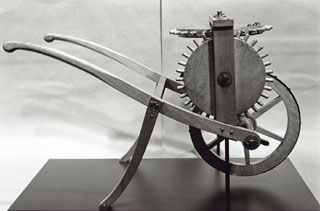
\includegraphics[width=70mm]{/content/DaVinciOdometer.jpg}
	  \caption{Da Vinci's mechanical pedometer}
\end{figure}


On-going progress is being made by various universities and institutes to address the issue of personal energy expenditure monitoring. This is due to the fact that the global economy is not able to meet the minimum conditions for sustainability. The Rio Declaration of 1992 and the United Nations Millennium Development Goals have demonstrated that human demand for ecosystem goods and services exceed the biosphere's total capacity. A fundamental solution is to manage food, fibre and energy consumption and maintain or increase the productivity of natural and agricultural ecosystems. From the number of proposed solutions, the 'shrink and share' framework has gained increasing recognition. This solution emphasises an equal allocation of emission rights to each person on the Earth and has been established by European Parliament as a basic principle for reducing global emissions of carbon dioxide [6].\\ \\
Simon Hay at University of Cambridge proposed a 'Global Personal Energy Meter' (PEM) device [7], which can record and apportion an individual's energy usage. The Architecture of this PEM would consist of a global sensor network and devices such as smartphones would communicate with it and receive estimates of energy used by individual. Data from a 'world model' (recommended energy usage allocations) would be fed into PEM to keep estimates up-to-date.\\ \\
Further research undertaken by Simon Hay, this time together with Stamatina Th. Rassia, Alastair Beresford and Nick V. Baker include 'Movement dynamics in office environment' [8] and 'Estimating personal energy expenditure with location data' [9]. The task of this research was to explore the relationship between indoor environments and physical activity by gathering location and physical activity data.


% Professional Considerations
\chapter{Professional Considerations}

\section{Code of Conduct}
The project is relevant to most of the sections in the Code of Conduct but one particular is highly relevant named Public Interest 1(a):\\ \\
\textit{"You shall have due regard for public health, privacy, security and wellbeing of others and the environment."}\\ \\
The implementation of Personal Energy Meter (PEM) requires use of the iPhone Location Services that gather location data of users. It must be assured that any storage or transfer of this data is secure and not leaked.\\ \\
Another important sections 2(a),(b), named Professional Competence and Integrity, mentioning the importance of not to claim that I know more than I do:\\ \\
\textit{"You shall only undertake to do work or provide a service that is within your professional competence."}\\ \\
\textit{"You shall NOT claim any level of competence that you do not possess."}\\ \\
This is particularly important as I am still a student with no full and certified competence.

\section{Code of Good Practice}
Although about 70\% of the document is closely related to this project it will be an excellent guide to ensuring that the project and any subsequent commercial work  is done correctly with highest possible quality.\\ \\
The development of this project must follow the Code of Good Practice particularly Section 4 which deals with Research and Section 5 which deals with Software Analysis, Design and Development. The study of this document will be included as a milestone in this project.


% Planning
\chapter{Planning}
As the nature of the project requires learning new programming languages, frameworks and toolkits, project becomes challenging and therefore there might be unexpected changes. This might require backtracking and re-designing the system and therefore an agile software development method called Scrum was chosen [10].\\ \\
The power of agile approach to software development is that a project does not need solid design before implementation stage but rather gathers and refines requirements through the development cycle. This is important phases in most of the today’s commercial projects. As economy changes rapidly, the project development cycle must be flexible enough to accommodate such changes to prevent wasting of resource.\\ \\
The opposite of agile is a software development method called waterfall. This method is a more solid sequence of procedures that don’t change much during the development cycle. Such methods are now mostly used for long term government projects or safety critical software where a safety and security have precedence over most current economy trends.\\ \\

The Scrum is a general agile method with focus on managing iterative development. There are three phases in Scrum:\\


\begin{figure}[H]
  \centering
	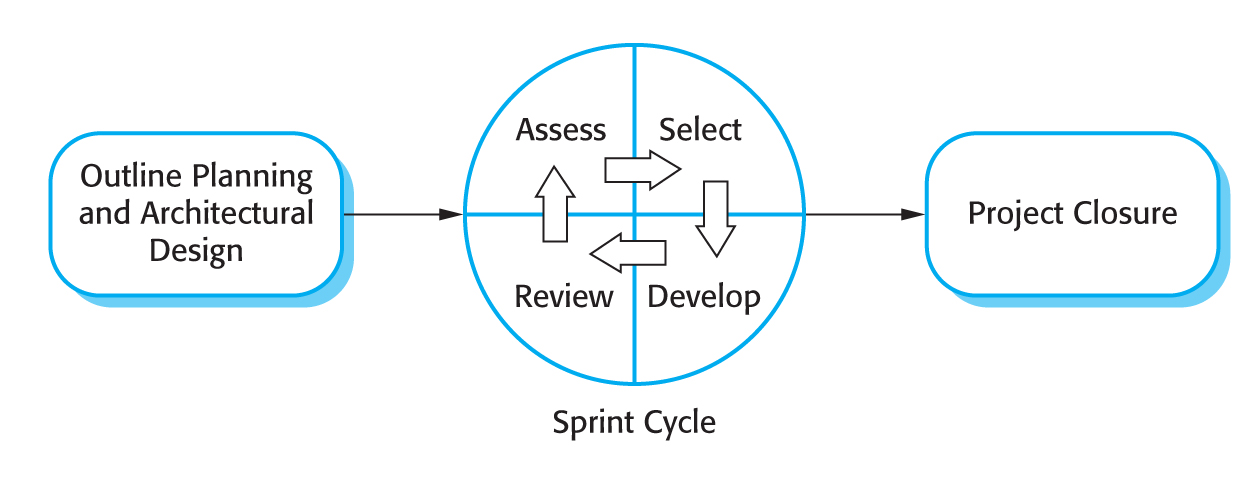
\includegraphics[width=120mm]{/content/SCRUM.jpg}\\
	  \caption{Scrum - the agile software development method.}
\end{figure}


\subsubsection{1. Outline planning and architectural design}
This phase was concerned with general objectives and requirement analysis for the project and with designing software architecture. The former requirements specification section was very detailed and less suitable for agile development and therefore data flow sections have been omitted. Most of the underlying functional requirements have been left unchanged, but there have been some additions or improvements to them as the project development progressed. Some features have been renamed to convey better meaning and for consistency. There was a need for PEM's user interface changes with subsequent knowledge of an iPhone development acquired.


\subsubsection{2. Sprint cycle}
A series of sprint cycles followed the previous phase where each cycle developed an increment of the system. Cycles had lengths of 1-4 weeks. At the beginning of each cycle, a meeting with a customer/supervisor took place where features of both applications were assessed and selected for development. The first half of the meeting was used for reviewing an already completed cycle. Details of the meetings in appendices show what has been assessed, selected and developed.


\subsubsection{3. Project closure}
The project closure phase wraps up the project, produces the required documentation and draws conclusions.


% Project plan
\clearpage
\section{Project plan}
\subsection{Project Outline}
The goal of the project is to develop a system that can estimate a user's caloric expenditure and advise them about their personal wellbeing or about the wellbeing of the planet.
The system is split into two parts. The first part is concerned with the development of the Personal Energy Meter (PEM), which is an iPhone application, and the second part is dealing with the development of a web application (PEMWEBAPP). The implementation of PEMWEBAPP has two purposes. Firstly, to receive data from PEM and present it in a better graphical way using full size of a computer monitor. Secondly, to demonstrate skills acquired during a course of study.


% Project schedule
\subsection{Project Schedule}
There are several important milestones in this project and each of them have several key tasks that must be performed. More information is given in the phase plan.
The main milestones for the project include:

\begin{itemize}
\item \textbf{General research} of the problem the project is concerned with, and production of the project plan overall (including the 
creation of this document as a guideline for the rest of the project, as well as being used 
as a general schedule). 



\item \textbf{Requirements Analysis}, aimed at finding all ambiguities, 
and determining exactly what the customer/user wants. This will include a decision on which 
design model to use.



\item \textbf{High Level Architectural Design}, which will help to determine how the applications will be structured given the limits and freedoms determined within the requirements Analysis phase.

\item \textbf{Implementation}, the stage in which the actual software systems are developed, using the designs created in the previous stage. This phase will overlap with a design phase throughout the whole development cycle to reflect on the agile approach.

\item \textbf{Evaluation of PEM} stage will be concerned with answering the questions whether the PEM solved the given problem, how well it solved it and how accurately the solution matches with requirements. 
\end{itemize}


% Phase plan
\subsection{Phase plan}
\subsubsection{General research}
\begin{enumerate}
	\item Literature reviews
		\begin{enumerate}
			\item Research materials about GPS systems
			\item Research materials about Accelerometer
			\item Research materials about human wellbeing by physical activity
			\item Research materials about human caloric expenditure
			\item Research materials about iPhone development and iOS SDK
			\item Research materials about Objective-C
			\item Research materials about Java EE 6, GlassFish  
			\item Research materials of British Computer Association
			\item Follow the book 'Projects in Computing and Information Systems'
		\end{enumerate}
	\item Meeting with customer/user
		\begin{enumerate}
			\item Meetings with project supervisor
			\item Getting feedback on application prototypes from friends
		\end{enumerate}
	\item Write the project proposal
\end{enumerate}


% Requirements Analysis
\subsubsection{Requirements Analysis - phase plan}
\begin{enumerate}
	\item Requirements discovery
		\begin{enumerate}
			\item User scenarios
			\item Customer/supervisor meetings
		\end{enumerate}
	\item Requirements classification and organization
		\begin{enumerate}
			\item Organising and clarifying what has been gathered from customer/users
		\end{enumerate}
	\item Requirements prioritisation and negotiation
		\begin{enumerate}
			\item Negotiating possible changes with customer/users and advise them on more suitable alternatives to meet the deadlines/budget
		\end{enumerate}
	\item Requirements specification
		\begin{enumerate}
			\item Clearing out ambiguities
			\item Producing a document which will act as a contract between customer and developer
		\end{enumerate}
	\item Write the interim report
\end{enumerate}


% Design
\subsubsection{Design - phase plan}
\begin{enumerate}
	\item PEM (Objective-C)
		\begin{enumerate}
			\item Architectural design for Profile manager
			\item Architectural design for Login with authentication
			\item Architectural design for Database (Apple's Core data)
			\item Architectural design for GPS tracking
			\item Architectural design for Live energy expenditure calculation
			\item Architectural design for Secure data transfer
		\end{enumerate}
	\item PEMWEBAPP (JavaEE)
		\begin{enumerate}
			\item Architectural design for Login with authentication
			\item Architectural design for Profile view
			\item Architectural design for Database (MySQL)
			\item Architectural design for sessions view
			\item Architectural design for session details view
			\item Architectural design for Statistics

		\end{enumerate}

\end{enumerate}


% Implementation and Testing
\subsubsection{Implementation - phase plan}
The aim is to start as soon as possible without having to wait for total completion of solid software design - hence the agile development model. Modularisation is used and attention is focused on some parts of the project, which will not change. In this way, implementation can start with only partial design. This strategy will be necessary in order to allow for any unforeseen complications in the design or implementation.
\begin{enumerate}
	\item Set up version control in Git
	\item PEM development
		\begin{enumerate}
			\item Implement Profile manager
			\item Implement Login with authentication
			\item Implement Database
			\item Implement GPS tracking
			\item Implement Live energy expenditure calculation
			\item Implement Secure data transfer
		\end{enumerate}
		Subtasks of the PEM development tasks will consist of:
		\begin{itemize}
			\item Interpreting architectural design diagrams in Objective-C language and trying to predict any deviations from the design.
			\item Coding the agreed design
			\item De-bugging
			\item Refactoring for better code structure
		\end{itemize}
	\item PEMWEBAPP development
		\begin{enumerate}
			\item Implement Login with authentication module
			\item Implement Profile view module
			\item Implement Database module
			\item Implement Statistics module
		\end{enumerate}
		Subtasks of the PEMWEBAPP development tasks will consist of:
		\begin{itemize}
			\item Interpreting architectural design diagrams in Java language and trying to predict any deviations from the design.
			\item Coding the agreed design
			\item De-bugging
			\item Refactoring for better code structure
		\end{itemize}
\end{enumarate}


% Evaluation
\subsubsection{Evaluation - phase plan}
\begin{enumerate}
	\item Evaluation of how well the systems meet customer/user requirement
		\begin{enumerate}
			\item There will be feedback received from the customer/user throughout the development process. Prototypes of the systems will be released in intervals to ensure meeting the requirements as closely as possible.
		\end{enumerate}
	\item Evaluation of how the systems are reliable
		\begin{enumerate}
			\item One of the extension features is to ensure the reliability of the PEM system by researching deep into iPhone Location Services and Accelerometer and utilizing full power of the hardware. The task of this part of evaluation will be proving the reliability of PEM in extreme conditions where two or more technologies might by interchanging in live energy expenditure monitoring mode.
		\end{enumerate}
	\item Evaluation of how the systems are accurate
		\begin{enumerate}
			\item In this part of the evaluation phase real biomedical results are obtained from health centres or fitness centers will be compared to those calculated by PEM. Results may be obtained on request from staff or by measuring caloric expenditure of myself on treadmill. Note that it is also one of the extensions and not a priority to complete project.
		\end{enumerate}
\end{enumerate}


% Evaluation
\subsubsection{Testing - phase plan}
Carry out unit tests at the end of each sprint cycle when design of the systems is likely to change.


% Time estimates
\subsection{Time estimates}
Activity-on-node diagrams below show estimates of the time to complete both PEM and PEMWEBAPP systems. The figures have been estimated with constraints of learning new programming language in mind.

\begin{figure}[H]
  \centering
	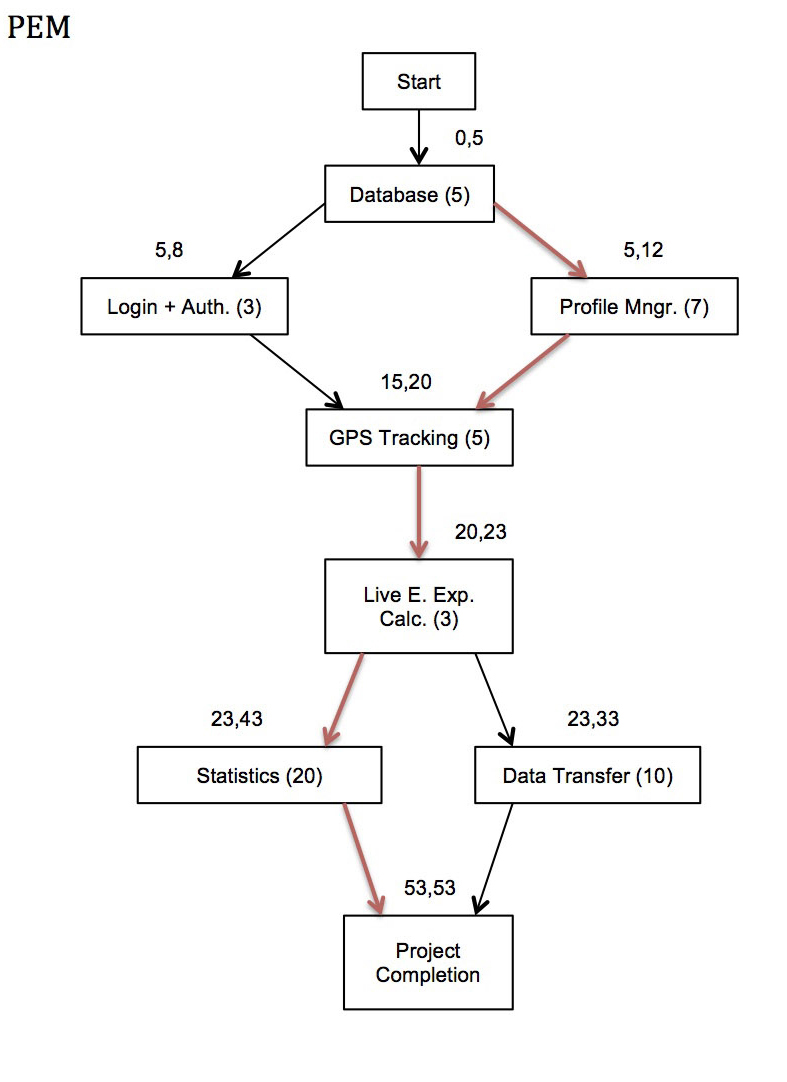
\includegraphics[width=120mm]{/content/PERTchart.jpg}
	  \caption{Activity-on-node diagram showing PEM development. Time granularity: days.}
\end{figure}

\begin{figure}[H]
  \centering
	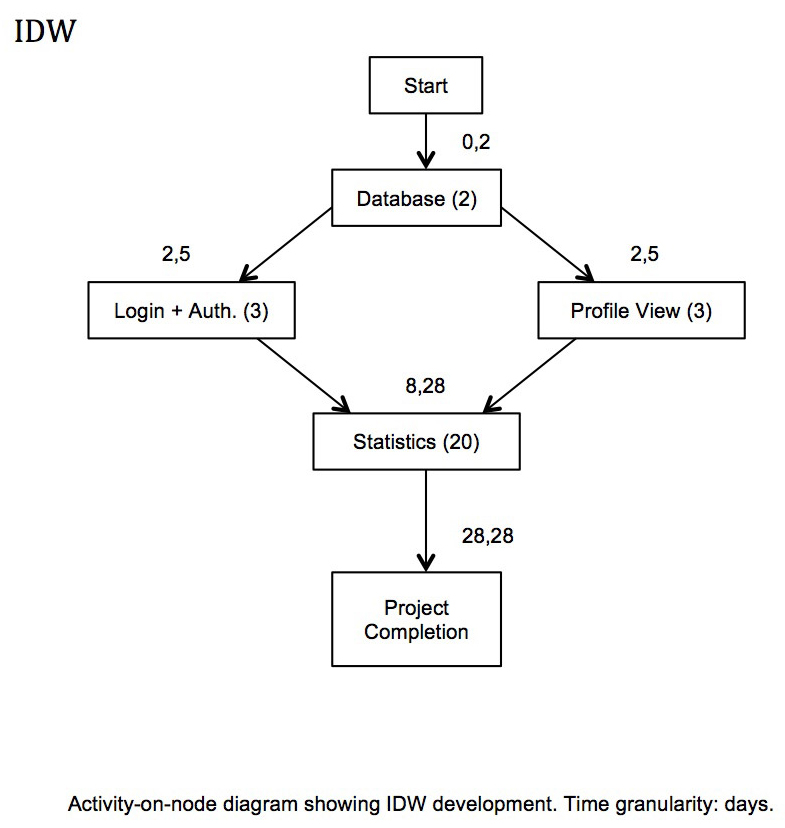
\includegraphics[width=120mm]{/content/PERTchart2.jpg}
	  \caption{Activity-on-node diagram showing PEMWEBAPP (formerly known as IDW )development. Time granularity: days.}
\end{figure}


% Requirements
\chapter{Requirements Analysis}

\section{Requirements discovery}
Requirements discovery has been carried out on three individuals. The project supervisor/main customer Martin and two friends, Tim and Richard. The requirements are very vague and high-level but refined throughout the stages of the Requirement Analysis.

\subsection{Collected scenarios}
\subsubsection*{Scenario 1}
Martin has a busy lifestyle in which time to rest and sleep is very precious. Therefore he would like to find a way of measuring and controlling the amount of energy he uses doing certain activities such as walking, running, cycling, working out in the gym or climbing stairs. As he is also very aware of the carbon footprint on the environment he would be interested in how much he could eliminate the emissions by changing his forms of transport.

\subsubsection*{Scenario 2}
Tim spends lots of hours in an office doing a sedentary job. To preserve his wellbeing he wants to know each day/week whether he had enough recommended physical activity. He would like to get accurate caloric expenditure results with healthy advice and recommendations directly on his iPhone or access them online via a web page where he can log in, see all the results collected, which would be graphically displayed using charts, and access and share other people's results to see general healthy trends.


\subsubsection*{Scenario 3}
Richard is a bodybuilder and therefore maintaining a strict workout program with enough rest each day is very important to him. As he is not a professional athlete he would appreciate some conventional way of keeping track of his caloric expenditure via heartbeat pulses while he works out in the gym. As a result, he would like to obtain very accurate data from which he could design or improve his workout program.

\section{Requirements classification and \\ organisation}
On examination of all three scenarios and after consideration of the resources available for undertaking the project, the following decisions have been made and presented to customer at one of the formal meetings: iPhone development will be used as this device was already available. (Developing for an iPhone also brings new challenges of learning new programming language, API and interesting development methods and models to this project.)

\subsubsection*{Product functionality}

The iPhone application should have the following functionalities:

	\begin{enumerate}
	\item Capture, categorise and process data (GPS, sound signal, accelerometer)
	\item Calculate caloric expenditure using an Metabolic Calculation Model Model
	\item Calculate a carbon footprint
	\item Graphically output the results of the calculations
	\item Give recommendations on personal and planetary wellbeing
	\item Send data to remote website
	\end{enumerate}

For accessing captured data from a computer an interactive dynamic website will be built. For the purposes of applying the knowledge of a Java language and Web Computing, the website will be coded using Java EE 6 which is the industry standard for enterprise Java computing. This website should have the following functionalities:
\begin{enumerate}
\item Create and maintain user profiles
\item Receive and process data from the iPhone application
\item Graphically output results of calculations
\item Give recommendations on personal and planetary wellbeing
\item Share personal energy expenditure data with other users
\item Energy expenditure trends visualisation (personal, carbon footprint)
\end{enumerate}
The classification and organisation of the requirements discovery was a first important step of translating the high level user's scenarios to more technical and measurable units.

\section{Requirements prioritisation and \\ negotiation}
Although the classification and organisation phase of the requirements discovery laid down some understandable structure to the project, which is closer to implementation than vague user scenarios, the time constraint of the project became very apparent. Negotiations with the customer therefore had to take place in order to preserve prototype and final product release dates schedule.

\subsubsection*{Objectives after negotiation}
Primary:
	\begin{enumerate}
		\item Design and develop the Personal Energy Meter (PEM), an iPhone application that 		should 	have following functionalities:
		\begin{enumerate}
			\item Capture and process GPS data of five activity domains (Walk, Run, Car, Bus and Train)
			\item Calculate caloric expenditure using an Metabolic Calculation Model Consumption Model
			\item Calculate a carbon footprint
			\item Graphically output results of the calculations
			\item Give recommendations on personal and planetary wellbeing
			\item Send data to remote website
		\end{enumerate}
		
		\item Design and develop an interactive website which should have following functionalities:
		\begin{enumerate}
			\item Create and maintain user profiles
			\item Receive and process data from the PEM, an iPhone application
			\item Graphically output results of calculations
			\item Give recommendations on personal and planetary wellbeing
		\end{enumerate}
	\end{enumerate}
Extensions: 
	\begin{enumerate}
		\item More precise GPS data processing by PEM
		\item Live GPS data categorisation (walking, driving car, running, using public transport)
		\item iPhone in-built headphones microphone integration for capturing the heartbeat (for estimating energy expenditure indoors where high volume of energy can be used for example in the gym or climbing stairs)
		\item Validation of the Energy Consumption Model with real biomedical measurements
		\item Improve accuracy and reliability of capturing the GPS data
		\item Share the personal energy expenditure data with other users
		\item Energy expenditure trends visualisation (personal, carbon footprint)\\
	\end{enumerate}
Splitting the project requirements, by negotiating with the customer, into two categories (Primary, Extensions) reduced a development overhead, which wasn't apparent in the initial stages of formal meetings. The negotiation gave both stakeholders a more clear understanding of what can be achieved within the designated time of the project (or how much the customer can have for what they paid). The development company has however offered the customer, for keeping good customer relations, implementation of some or all 'Extensions' if time allows.


% Requirements Specifications
\section{Requirements Specification}
Requirements have been captured in a Requirements Document (RD), which forms an official statement of what the system developer (myself) should implement.\\ \\
PEM is a small iPhone application that solves the problem of knowing a person's energy expenditure in everyday life. It monitors a person's movement and, from data obtained, it estimates the amount of calories a person has burned in various activities. As an output, PEM provides a graphically aided representation of results together with healthy recommendations. PEMWEBAPP is a website which solves a problem of having to interact with limited size of an iPhone screen and present the results in better graphical way on computer monitor.

\subsection{User requirements definition}
The PEM shall create a user profile and shall provide a profile view where updating a user's profile data is possible. The PEM shall provide GPS tracking for five activity domains (Walk, Run, Car, Bus and Train) and shall calculate caloric expenditure and carbon footprint, and shall have an option to save the activity tracking as a session into persistent store for later retrieval. The PEM shall have a session details view where retrieved information will be displayed and emphasised by graphical aids. The PEM shall have an upload feature for uploading the data (profile and sessions) into online PEMWEBAPP. The PEM shall provide recommendations on personal and planetary wellbeing and have user authentication feature.\\ \\
The PEMWEBAPP shall manage user profiles, display profile and profile's sessions (recordings of monitored activities) and shall provide sessions details view. The PEMWEBAPP shall provide a delete profile button for deletion of the profile and all its sessions. The PEMWEBAPP shall also have a statistics view where each session will be depicted on a line chart showing caloric expenditure and carbon footprint data. The PEMWEBAPP shall provide recommendations on personal and planetary wellbeing and have a user authentication feature.


\begin{figure}[H]
  \centering
	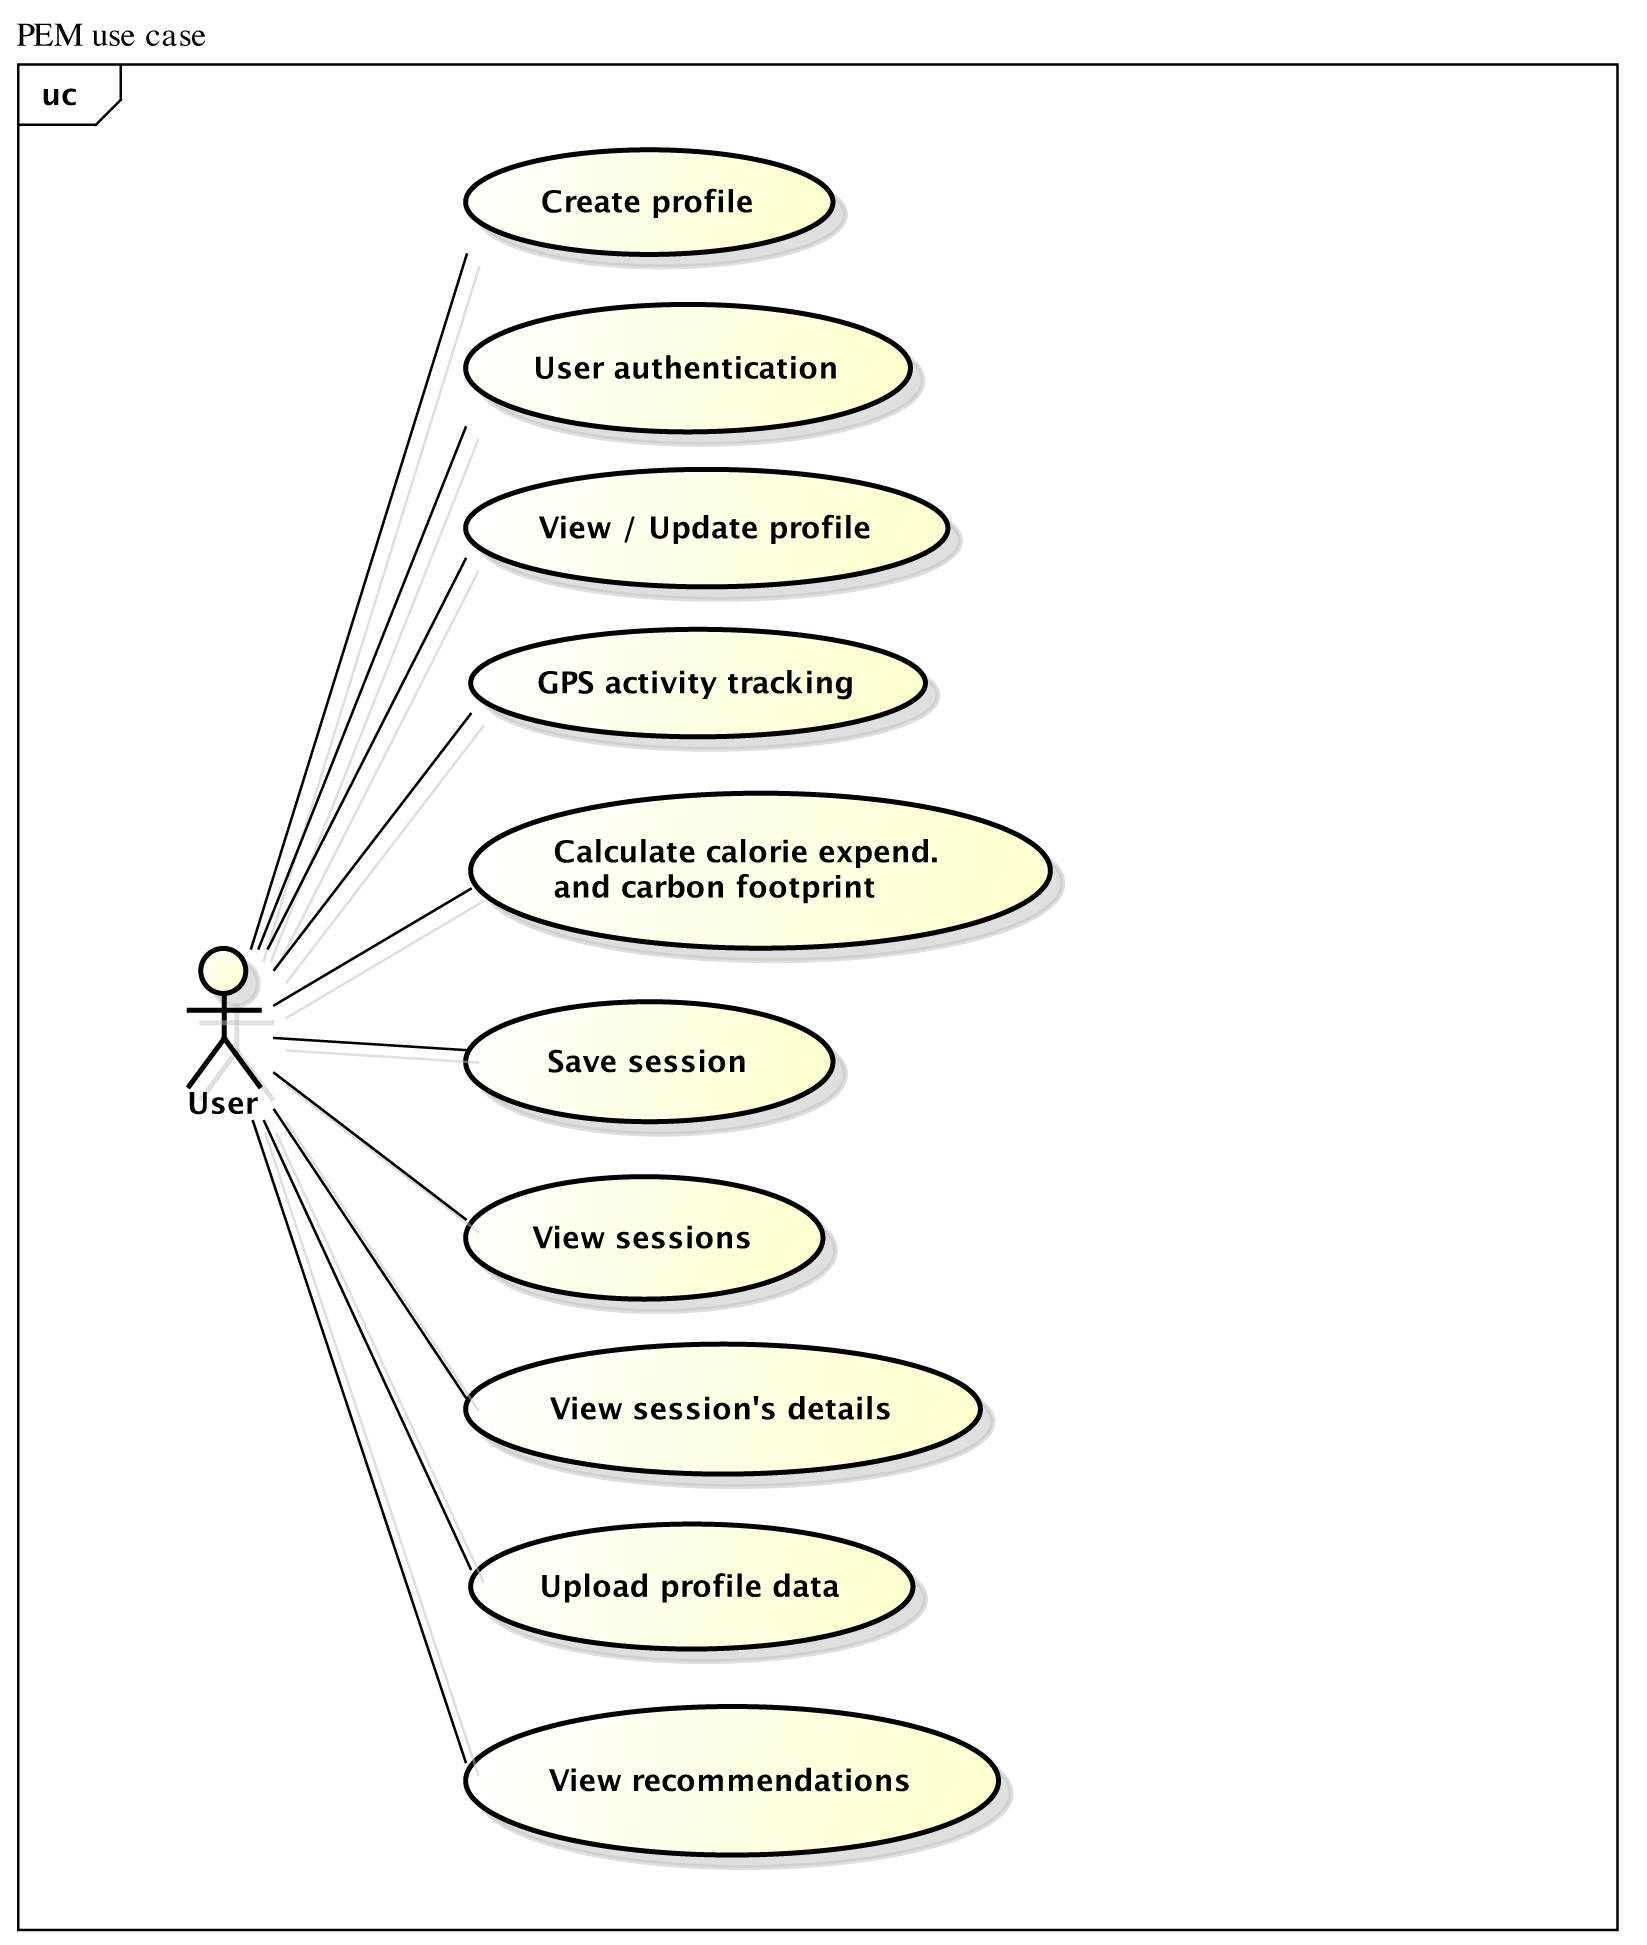
\includegraphics[width=120mm]{/content/PEM_use_case.jpg}
	  \caption{PEM's use case}
\end{figure}

\begin{figure}[H]
  \centering
	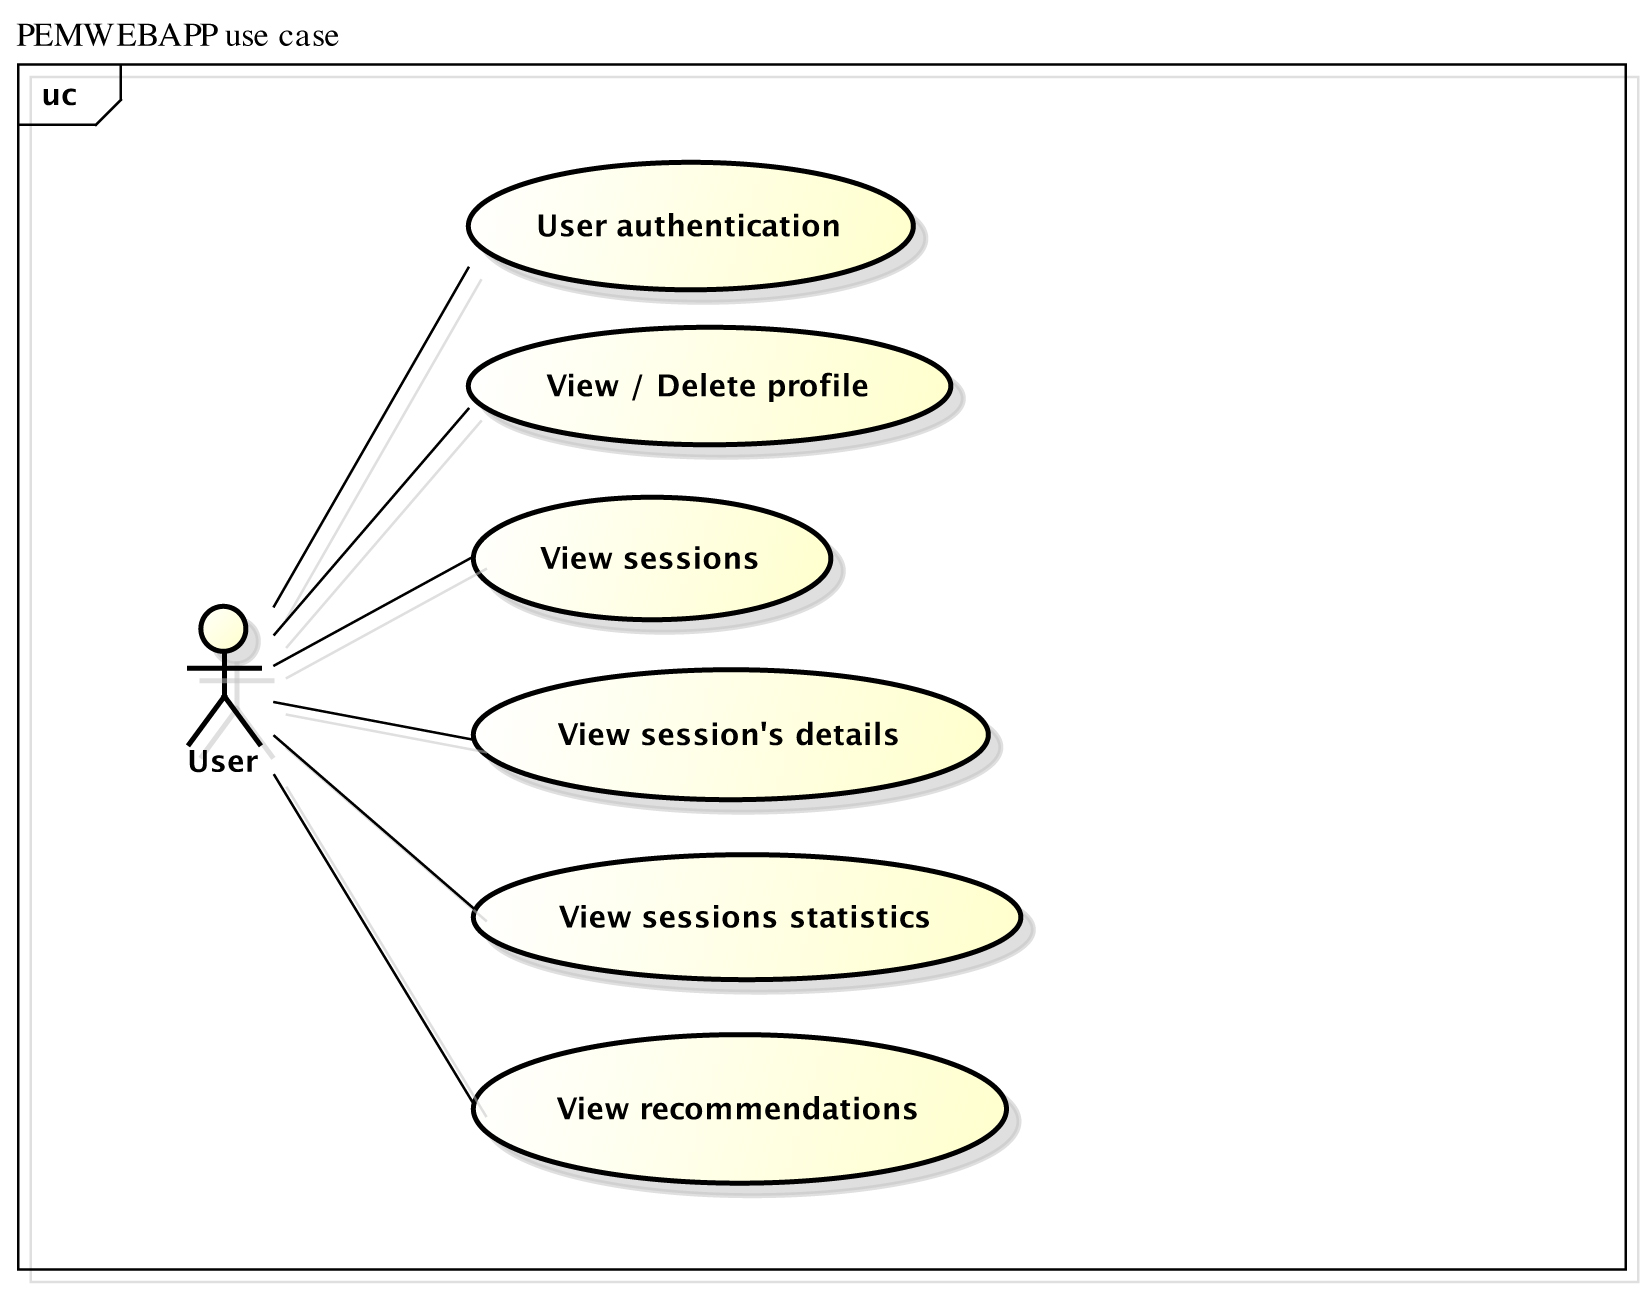
\includegraphics[width=120mm]{/content/PEMWEBAPP_use_case.jpg}
	  \caption{PEMWEBAPP's use case}
\end{figure}


% Functional requirements
\subsection{System requirements specification}
\subsubsection{Functional requirements}
Personal Energy Meter (PEM)\\ \\
\textbf{1. Create Profile}\\
This feature shall provide the ability to create a new profile on the PEM. It is the first thing a user must do to begin using PEM. Its main function is to set up a new profile with personal details such as email and password. Email shall act as a username and must be unique. The password must be at least 4 characters long, no longer than 20 and must contain at least one numeric character. No special characters are allowed.\\ \\
\textbf{2. Log-in}\\
This feature shall allow the user to log in to the existing profile on PEM. When choosing to log in, the user is asked to enter their email and password. After a successful authentication the activity screen appears.\\ \\
\textbf{3. Edit profile}\\
This feature shall allow the user to edit their personal details on PEM. When the user is logged in they should be able to edit they personal details such as adding the first and second name or change their body weight. There shall be a constraint on editing the email to preserve correct transfer of data to the appropriate profile on the remote server (email is unique and represents a profile). The password must be at least 4 characters long, no longer than 20 and must contain at least one numeric character. No special characters are allowed.\\ \\
\textbf{4. Delete profile}\\
This feature shall allow the user to delete their profile from the PEM. Users not wanting to keep their profile for various reasons or wanting to start from scratch should have an option to delete their profile with all the data gathered. This operation should only affect the PEM system. Users should be able to still access their profile online to see all of the data and results. Deleting an online profile shall be done in the PEMWEBAPP.\\ \\
\textbf{5. Start tracking}\\
This feature shall allow the user to start their energy expenditure or carbon footprint monitoring. By pressing the Start button, the iPhone device shall start to receive GPS data and at the same time shall perform live calculations of calories burned and/or CO$_{2}$ emissions calculations. The Location Services on iPhone have to be enabled in order for PEM to receive any GPS data.\\ \\
\textbf{6. Stop tracking}\\
This feature shall allow the user to stop their energy expenditure or carbon footprint monitoring as well as to stop receiving GPS data. By pressing the Stop button, the user should be prompted if they whish to save a session. Monitoring needs to be in progress in order for Stop to have an effect and ask about saving the data.\\ \\
\textbf{7. Pause tracking}\\
This feature shall allow the user to pause their energy expenditure or carbon footprint monitoring as well as to stop receiving GPS data and resume it all again.\\ \\
\textbf{8. Google maps and tracking information}\\
This feature shall the allow user to see their live position on Google maps and GPS data as they are received in intervals (every second). Data such as horizontal accuracy, elevation, distance traveled, grade, speed, time, VO$_{2}$, Calories and CO$_{2}$ emissions should be displayed under map view. The map view should be zoom-able and follow the user's current position.\\ \\
\textbf{9. Sessions view}\\
This feature shall allow the user to navigate through all saved sessions (related to their profile) and choose their desired session to show in the details view. This view shall pull limited session data from the PEM's database to show only a session name and timestamp. User should be able to delete the session from this view by swiping the session cell or by using an edit button.\\ \\
\textbf{10. Session details view}\\
This feature shall allow the user to see session details. The view shall contain all information gathered by GPS tracking and also results of calculations (session name, timestamp, activity, horizontal accuracy, elevation, distance traveled, grade, speed, time, VO$_{2}$, Calories and CO$_{2}$ emissions). The most important data, such as total caloric expenditure or total CO$_{2}$ emissions should be emphasised using graphical aids.\\ \\
\textbf{11. Recommendations}\\
This feature shall provide the most important information and facts about a type of activity monitored. For example if the Walk or Run activity has been monitored and stored the feature should provide relevant information about recommended daily amount of calorie intake and guidelines on how to lose or maintain weight. For sessions, which monitored activity such as Car, Bus or Train, recommendations should advise users about ways on how to reduce carbon footprint.\\ \\
\textbf{12. Upload profile}\\
This feature shall upload user's profile with all sessions to the remote PEMWEBAPP. This operation should be available at any time after the user profile has been created.\\ \\
\textbf{13. Log-out}\\
This feature shall log user out from the PEM.\\ \\
\subsubsection{Functional requirements}
PEM Web Application (PEMWEBAPP)\\ \\
\textbf{1. Log-in}\\
This feature shall allow the user to log in to the existing profile on PEMWEBAPP. When choosing to log in, the user is asked to enter their username and password. After a successful authentication a profile view appears.\\ \\
\textbf{2. Profile page}\\
This feature shall allow the user to see their profile. Information such as first and last name, email address and body weight should appear as the user entered them in the PEM. The password shall not show in this view. None of the information shall be editable.\\ \\
\textbf{3. Delete profile}\\
This feature shall allow a user to delete their profile from the PEMWEBAPP. Users can delete unwanted profile together with all the data gathered. This operation can't be undone.\\ \\
\textbf{4. Sessions page}\\
This feature shall allow the user to navigate through all uploaded sessions (related to their profile) and choose the desired session to show in the details view. The view shall pull limited session data from the PEMWEBAPP's database to show only a session name and timestamp. None of the information shall be editable.\\ \\
\textbf{5. Session details page}\\
This feature shall allow the user to see session details. The view shall contain all information as they were stored by PEM (session name, timestamp, activity, horizontal accuracy, elevation, distance traveled, grade, speed, time, VO$_{2}$, Calories and CO$_{2}$ emissions).\\ \\
\textbf{6. Statistics page}\\
This feature shall allow the user to see statistics of recorded activities in a line chart. The line chart shall show Calories burned and CO$_{2}$ emissions for each session.\\ \\
\textbf{7. Recommendations}\\
This feature shall provide the most important information and facts about a type of activity monitored (very similar to PEM's recommendation feature with exception that it should be accessible from the statistics page rather than session details page).\\ \\
\textbf{8. Log-out}\\
This feature shall log the user out from the PEMWEBAPP.\\ \\


% Non-functional requirements
\subsubsection{Non-functional requirements}

\begin{enumerate}
	\item Product requirements\\ \\
	The following are the Human-Computer-Interaction guidelines against which the PEM application should be evaluated. PEMWEBAPP should be also evaluated against these guidelines where appropriate.\\
	\begin{enumerate}
		\item Usability goals
		\begin {enumerate}
			\item Effectiveness: energy and caloric estimates must be of reasonable accuracy for the application to be effective. The results of the estimates should not be different by more than 20\% from current standards.
			\item Efficiency: the application needs to have immediate response and perform live calculations 
			\item Safety: safe storage and data transfer is critical for this type of application and users should not have to worry whether their data is safe.
			\item Utility: PEM should be built correctly and do only what is its intention to maximize utility. There should be no adverts or misleading content.
			\item Learnability: PEM must be easy to learn. Following Apple's Human Interface guidelines, the Norman's design principles and using well identifiable buttons and other UI controls will be necessary to achieve this. Furthermore, the application must be simple to use for users who are complete novices. It must have step-by-step instructions for initial setup, tracking and profile upload. Option selection should be constrained to prevent wrong choices. There is no need for extra flexibility or shortcuts for advance users because the PEM will be very easy to use with a limited number of features.
			\item 6. Remembering: PEM will be a multiscreen application. To maximize recognition rather than recall, each screen will have unique elements wrapped into consistent design used throughout the application.\\
		\end{enumerate}

		\item Experience goals
		\begin{enumerate}
			\item Satisfaction: the PEM should invoke a satisfying feeling when it proves itself effective.
			\item Enjoyment, Fun and Entertainment: PEM should strive for this goal by using simple, responsive and swift GUI. The session details view could be a good place to invest in creativity.
			\item Helpfulness: PEM should deserve this goal by being reliable and delivering correct data when needed. Users then can make wise decisions based on the application's recommendations.
			\item Motivation: PEM should be able to motivate people to reduce carbon footprint and motivate them to live healthily.
			\item Aesthetic: PEM should have aesthetic qualities if the design will follow the design principles and human interface guidelines.
			\item Support: PEM should have a help section which is easy accessible and readable.
			\item Reward and Emotional fulfillment: Users of PEM should be able to feel rewarded and emotionally fulfilled for helping to improve their health and planetary wellbeing.\\
		\end{enumerate}
		
		\item User Interfaces:
		\begin{enumerate}
			\item PEM user interface shall be made of various forms, views and pickers all of which are standard iPhone UI components. It should consist of the following screens (Login, Activity, Profile, Tracking, Save session, Sessions and Session details). A tab bar at the bottom of the GUI will allow switching between individual screens.\\
			\item PEMWEBAPP user interface shall be made of Java Servlet Faces and third party PrimeFaces components, which support AJAX for better user experience. It should consist of the following pages (Login, Profile, Sessions, Session details and Statistics). To navigate through the website, standard top-horizontal navigation consisting of links shall be used.\\
			\end{enumerate}
	
		\item Efficiency requirements
		\begin{enumerate}
			\item PEM's monitoring feature should be able to pin point most accurate current position within 10-20 seconds outdoors.\\
			\item iPhone's inaccurate altitude data received from GPS shall be replaced with accurate elevation data. For this purpose the Google Elevation API shall be used.\\
		\end{enumerate}

		\item Security requirements
		\begin{enumerate}
			\item Both applications shall use hashing of stored data.
			\item Use secure data transfer.
			\item Use user authentication.\\
		\end{enumerate}
	\end{enumerate}

	\item Organisational requirements

		\begin{enumerate}
			\item Platforms and languages
			\begin{enumerate}
				\item PEM - Apple (Objective-C)
				\item PEMWEBAPP - Oracle (Java Enterprise Edition)
				\item PEM - SQLite database wrapped by Core Data
				\item PEMWEBAPP - MySQL database\\
			\end{enumerate}
			
			\item Interoperability
			\begin{enumerate}
				\item PEMWEBAPP shall be implemented as a REST service so that iPhone can communicate with it using GET and POST commands.\\
			\end{enumerate}

			\item Metabolic and carbon footprint calculations
			\begin{enumerate}
				\item PEM shall make use of the ACSM's Metabolic Calculation Handbook for calculating VO$_{2}$ and consequently calculating of caloric expenditure.
				\item PEM shall make use of the Carbon Trust's passenger transport conversion factors for calculating carbon footprint.\\
			\end{enumerate}
		\end{enumerate}
		
		\item External requirements
		\begin{enumerate}
			\item The PEM must be built correctly to pass Apple's requirements for application distribution in the App Store. Both PEM and PEMWEBAPP must comply with the Code of Conduct and the Code of Good practice and must use secure file transfer to online website, cannot violate personal privacy by broadcasting user's location and location history must be stored securely.
		\end{enumerate}
	\end{enumerate}
	

% System models
\subsection{System models}
The following models are activity diagrams of both applications. The first diagram was created in the initial stages of the development where as the second diagram was created in later stages of the development when more knowledge and experience have been acquired.


\begin{figure}[H]
  \centering
	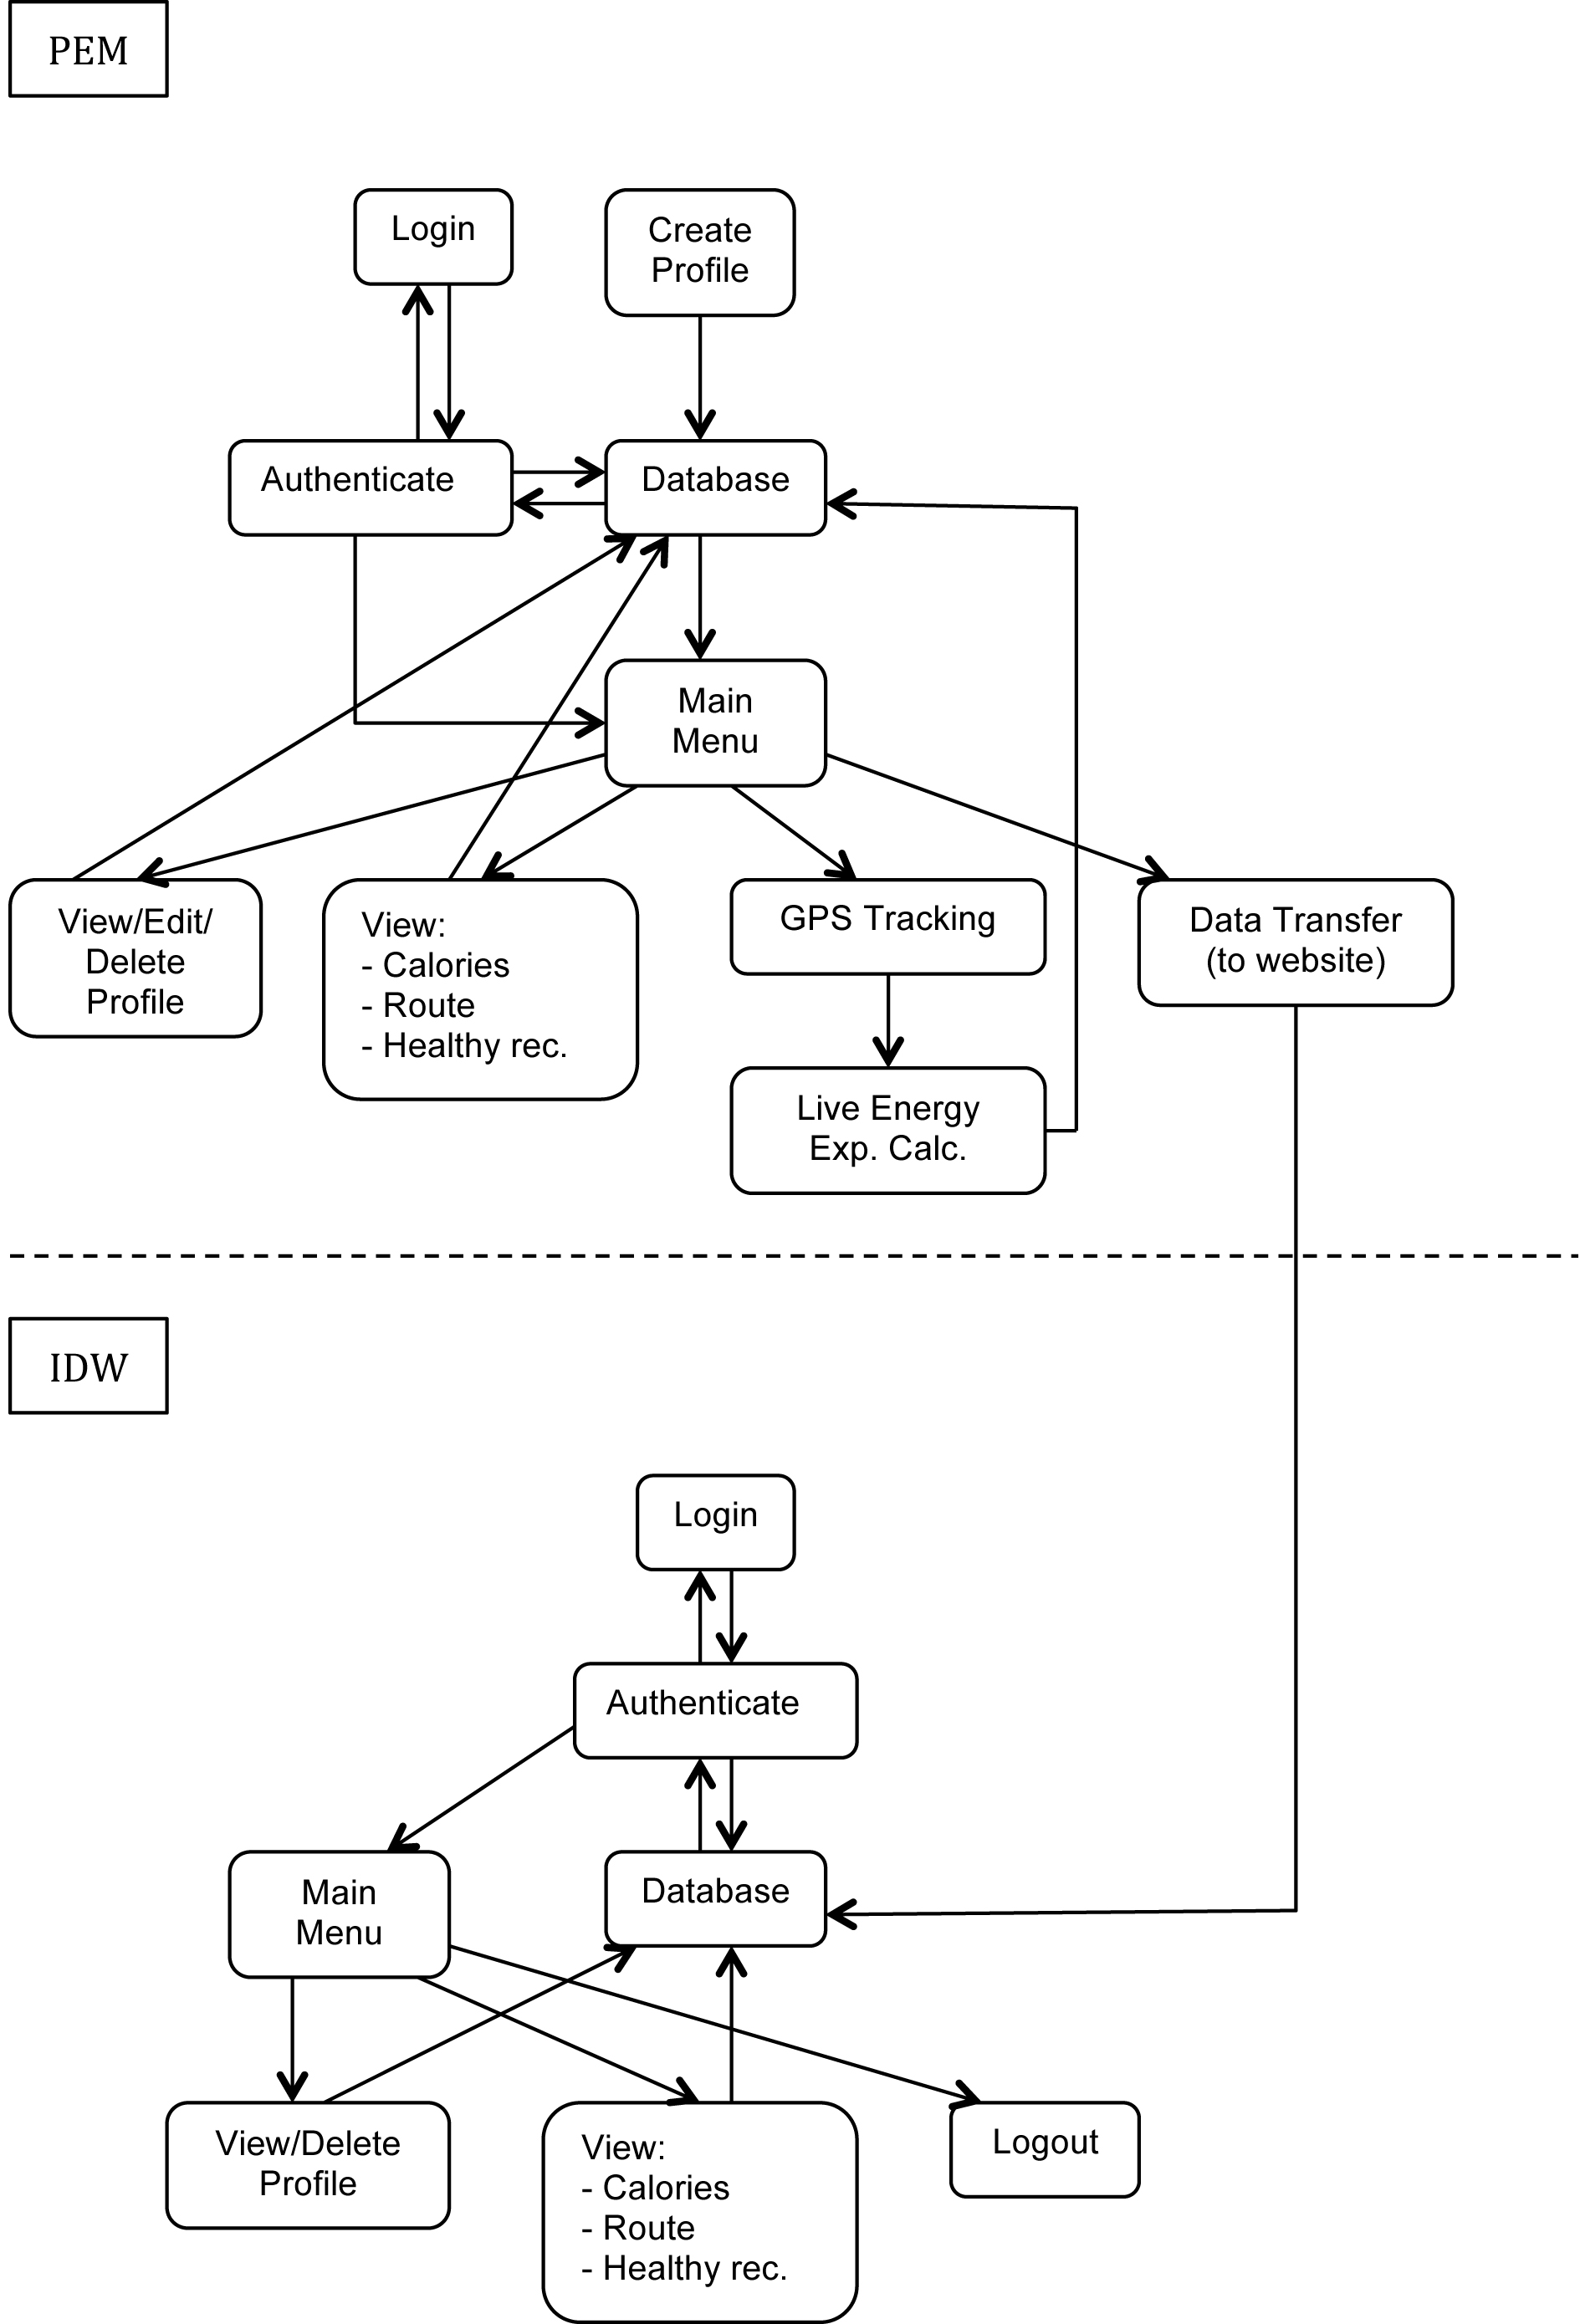
\includegraphics[width=120mm]{/content/InitialObjectDiagram.jpg}
	  \caption{The initial object diagram showing interactions between the PEM and the IDW (aka. PEMWEBAPP).}
\end{figure}


 \begin{figure}[H]
 \begin{sideways}
 \begin{minipage}{19cm}
	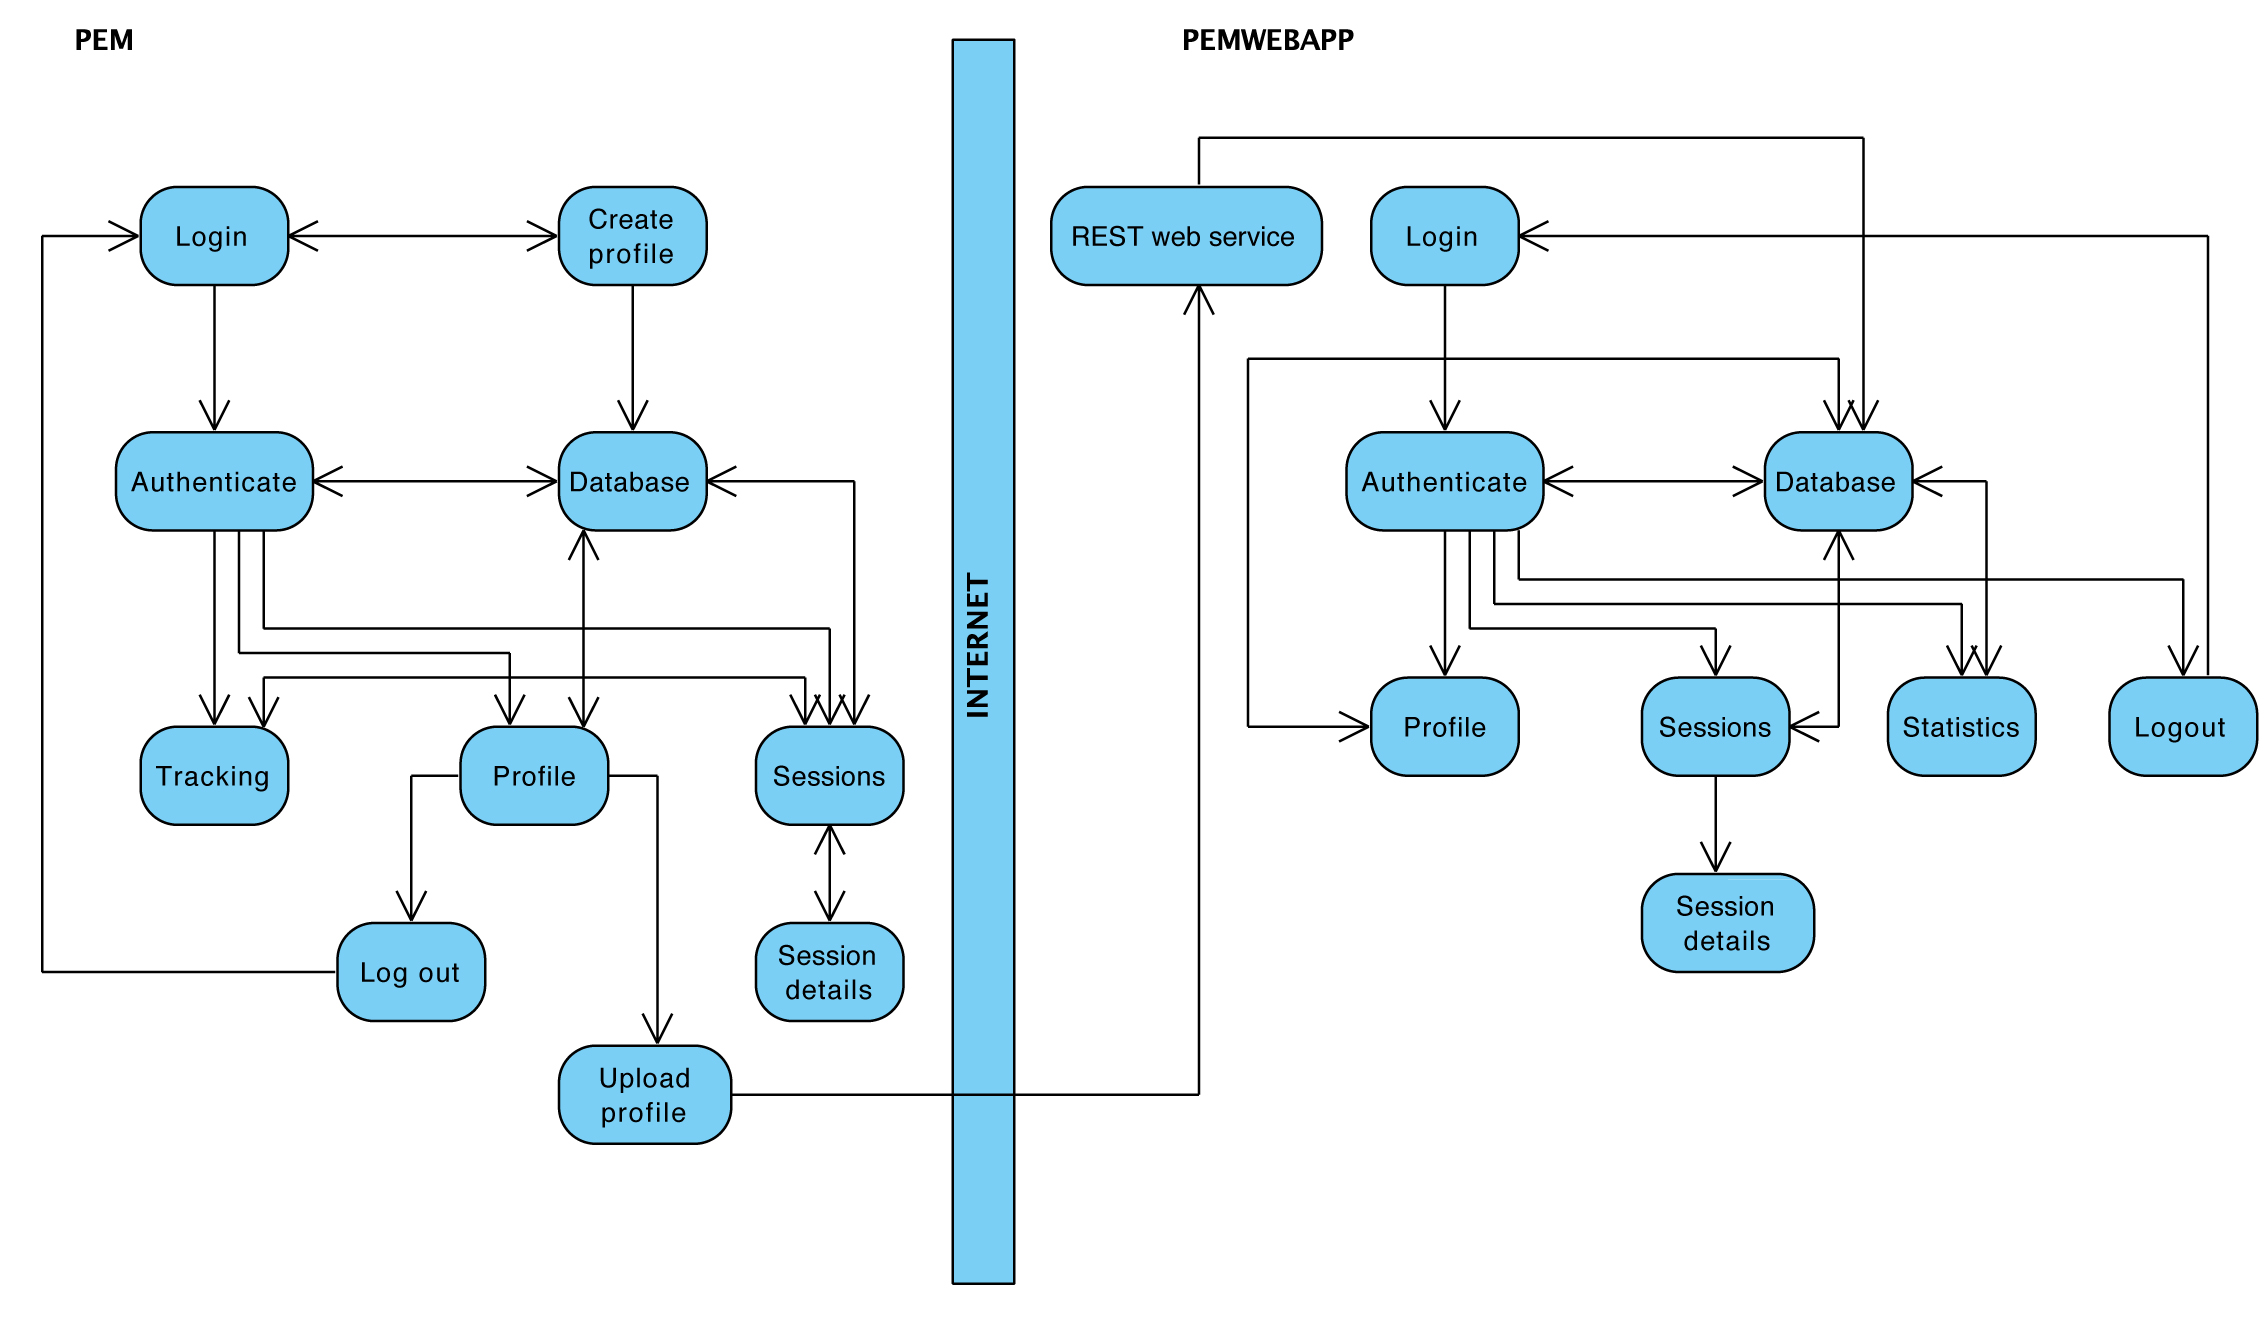
\includegraphics[width=200mm]{/content/SystemsObjectDiagram.jpg}
	  \caption{Improved object diagram showing interactions between the PEM and the PEMWEBAPP in mid stages of the development.}
 \end{minipage}
 \end{sideways}
 \centering
 \end{figure}


% Design and Implementation
\chapter{Design and Implementation}
\section{Introduction}
As already mentioned, the agile software development was most appropriate for this project and therefore there was no solid design in the initial stages of PEM and PEMWEBAPP development.
The design was being developed continuously by getting ideas, proposing solutions, and refining these solutions as information became available. On many ocassions there was a need to backtrack and re-design when problems arose. Paper sketches and Xcode's storyboards were the only key documents from which the development initiated. There was a time when the vast majority of the PEM had to be redesigned as knowledge of iPhone development improved and having a detailed design beforehand would be a waste of time.\\ \\
Some inspiration of how the PEMWEBAPP might look like or what data might be useful to collect came from fitbit.com and bodymedia.com. Both companies are well established in areas of estimating personal energy expenditure.

\begin{figure}[H]
  \centering
	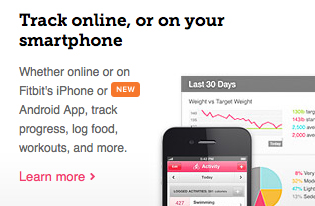
\includegraphics[width=120mm]{/content/fitbit.jpg}
	  \caption{One of the features promoted by Fitbit.com.}
\end{figure}

\begin{figure}[H]
  \centering
	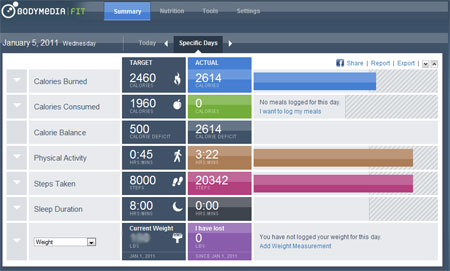
\includegraphics[width=120mm]{/content/bodymedia.jpg}
	  \caption{Dynamic website of Bodymedia.com.}
\end{figure}

\clearpage
\section{Building a simple iPhone application}
The project has initiated by initial meeting, which focused on a chosen project topic. The discussion covered available hardware and software and was aimed at encouraging a new programming language to be learnt. The first stage of the Scrum method, the planning, included gathering requirements, getting to know an iOS development and Xcode IDE, registering in an Apple Developer Program and configuring a computer to be able to deploy applications to an iPhone. The first sprint cycle was launched as soon as basic knowledge of an iPhone development was acquired and some requirements gathered, resulting in creation of a simple iPhone application.

\begin{figure}[H]
  \centering
	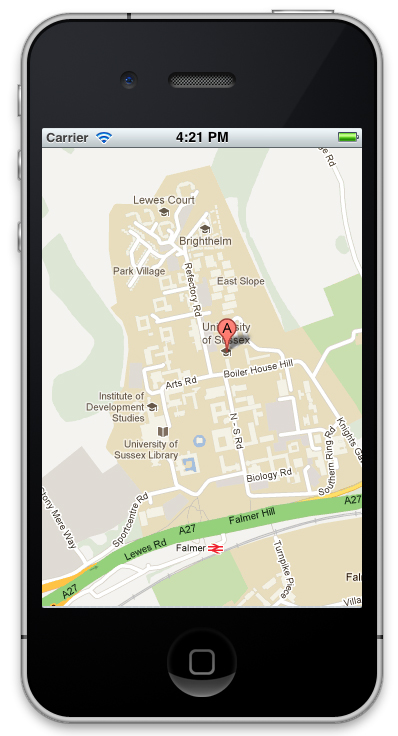
\includegraphics[width=50mm]{/content/simpleiPhoneApp.jpg}
	  \caption{Simple iPhone application.}
\end{figure}


The application was able to pinpoint a user's current position and show it in a map view. To build this simple application a fundamental iPhone development design pattern had to be used, the Model-View-Controller (MVC) pattern. The MVC is a software architecture pattern, which splits the application’s interaction into three parts. The Model deals with business logic (handling a data stored in database), View deals with the user interface and controller deals with how user interacts with the application (all of the application’s functionality). The pattern is popular in software development because it decouples the application so changes to the code can be done easier in future. \\ \\
A view was built in the Xcode's Interface Builder and wired up to the application's logic. This logic was written in an ordinary class, which was a subclass of a UIViewController (User Interface View Controller) providing more functionality. At this stage there was no mechanism to persist application's data thus the Model part of the MVC pattern wasn't fully utilised. Figure~\ref{iOSAppKeyObjects} and~\ref{iPhoneApp-wiringAction} below show iPhone's application key objects and how the functionality was wired up to the user interface.


\begin{figure}[H]
  \centering
	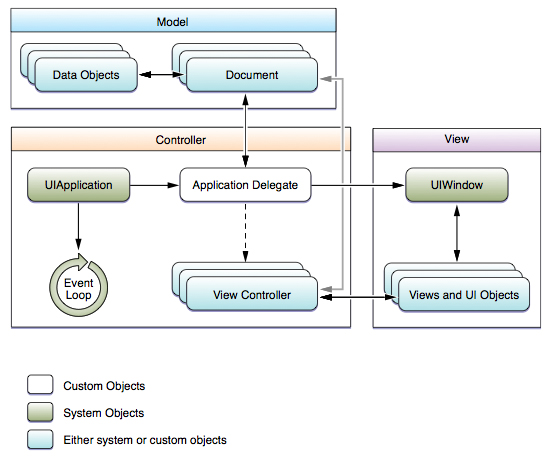
\includegraphics[width=120mm]{/content/iOSAppKeyObjects.jpg}
	  \caption{Apple programming guide [11].}
	  \label{iOSAppKeyObjects}
\end{figure}

\begin{figure}[H]
  \centering
	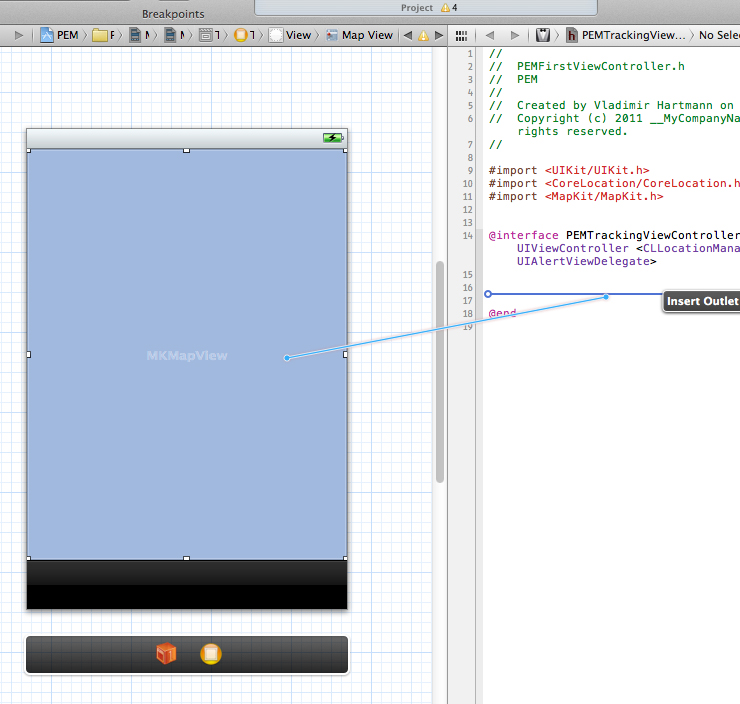
\includegraphics[width=100mm]{/content/iPhoneApp-wiringAction.jpg}
	  \caption{Wiring up functionality to user interface.}
	  \label{iPhoneApp-wiringAction}
\end{figure}


\clearpage
\section{Improving the simple iPhone application}
Demonstration of the simple iPhone application to the customer/supervisor completed the first sprint cycle and at the same time initiated the next sprint cycle with emphasis on writing as much code as possible without worrying about detailed design. Main tasks of this cycle were further programming of the simple iPhone application, research of previous attempts to build PEM, study of Apple's Human-Interface guidelines and gathering literature about utilising location services on iPhone and about GPS in general. As a result a GPS application was built that could capture location coordinates of current position and display them on iPhone screen.


\begin{figure}[H]
  \centering
	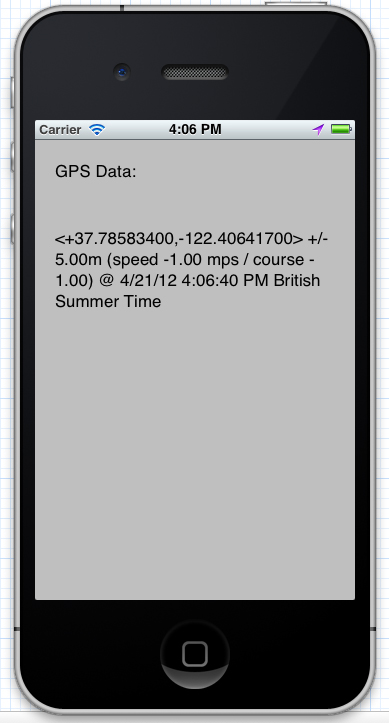
\includegraphics[width=50mm]{/content/FirstGPSApp.jpg}
	  \caption{The simple iPhone application extended by GPS functionality.}
\end{figure}


\clearpage
\section{Utilizing Apple's Core Data and Core Location}
The following two sprint cycles were mostly concerned with learning iPhone data persistence and location services.

There are many ways how to persist data on iPhone devices such as using property lists, archiving, directly interfacing with SQLite or using the Core Data framework. The first two approaches were not very suitable for storing big amounts of data. Utilising the SQLite and directly interfacing it would work just fine, but Apple introduced a more elegant solution of working with relational databases. Core Data allows the programmer to think of their data model in terms of objects/entities and their relationships. This is important as the code can retrieve and manipulate this data on a purely object level with simplified fetch requests and there is no need to work with relation schemas and complicated query language which can introduce errors or security issues.
Because receiving location data is not enough to estimate user's caloric expenditure, it was necessary to learn about Core Location.
Core Location is an iOS framework which allows easy access to the iPhone's GPS. The precise Apple's description is:
"The Core Location framework lets you determine the current location or heading associated with a device. The framework uses the available hardware to determine the user's position and heading. You use the classes and protocols in this framework to configure and schedule the delivery of location and heading events. You can also use it to define geographic regions and monitor when the user crosses the boundaries of those regions." [12]\\ \\
It is important to mention that during assessments and reviews of these sprint cycles discussion on how to improve accuracy was also relevant. GPS hardware in Apple's devices as well as in any other mobile device currently on market is well known for producing inaccurate altitude data. This is mostly due to position of satellites, which calculate the altitude.\\ \\
One of the suggested project extensions was the implementation of signal processing for heart beat measurements. This technique, if implemented correctly, would prove very accurate for estimating caloric expenditure as it could be used in situations where a user's position is not changing much but caloric expenditure is high e.g. working out in a gym. The signal processing approach is a big subject on its own and soon became apparent that the realisation of this technique would need far more time than allocated for the final year project.\\ \\
At the end of the cycles a first PEM prototype was built which featured everything previously built so far, plus the ability to measure the distance. Extensive GPS data filtering had to be done in order to work with the gathered data. For example, lots of invalid location data was received during Core Location initialization with values differing up to 500m. These had to be filtered out by checking their timestamps or specifying a threshold. Core Location uses caching for storing previously gathered data to prevent frequent use of the GPS. For real time application such as PEM however, this would cause old data to be processed in later implemented calculations. A compromise had to be made to trade battery life for up-to-date data.


\begin{figure}[H]
  \centering
	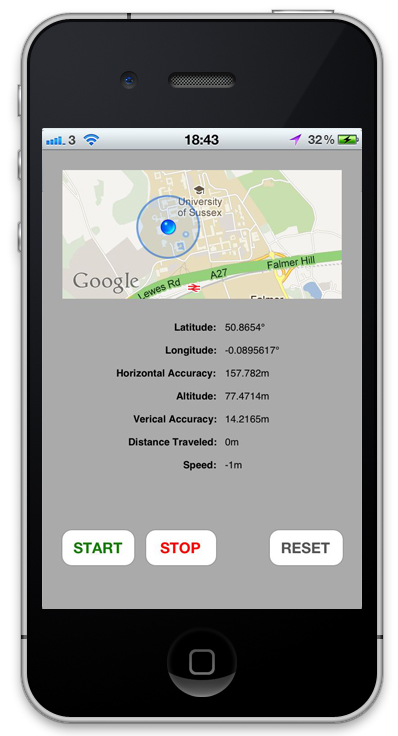
\includegraphics[width=50mm]{/content/PEM-firstPrototype.jpg}
	  \caption{The First PEM prototype.}
\end{figure}


\clearpage
\section{Building a multi-view iPhone application}
From this point on in the development of the PEM the sprint cycles spanned through up to 4 weeks. Communication was done mostly via emails and meetings took place once a month on average. This was due to increasing complexity of implementing new features and other factors such as coping with workload from other course modules.\\ \\
The fifth sprint cycle was mostly concerned with building graphical user interface (GUI) and migrating from Xcode 3 to Xcode 4.\\ \\
With a purchase of a new MacBook Pro, there was a possibility to run the newest software, which was previously impossible due to the old computer. Xcode 4 was a major re-write of this Interactive Development Environment and introduced new ways of creating iPhone applications. A feature of storyboards added to Xcode's Interface Builder (IB) enormous power as the GUI could be built from multiple views placed on a single IBs canvas resulting in more streamlined development. The Xcode migration was somewhat challenging though. Any prior knowledge of iPhone development wasn't fully compatible with the new version of Xcode and new knowledge of the same fundamentals already learned had to be acquired. This unexpectedly slowed down the development, which got back to normal when new techniques learned proved more efficient.\\ \\
As the knowledge of iPhone development improved, in addition to MVC, concepts such as delegation and protocols had to be utilised in order to establish communication between multiple views or creating custom iPhone functionality.\\ \\
Delegation can be thought of as a design pattern. In the world of iPhone development it can be explained as follows. Apple designs some basic, standard functionality for example for how the iOS should respond to user's actions. This functionality is defined in some class e.g. UIViewController which can be thought of as a protocol. Developers of iPhone applications can make use of this protocol by declaring it in a custom class they are developing. All UIViewController functionality will now be delegated to this custom class. Developers can now use all that functionality without writing any code or building on top of it to make more sophisticated behaviour. Using a delegation is a recommended standard and is inevitable for building correct iPhone applications.\\ \\
The result of the fifth sprint cycle was a PEM prototype extended by multi view functionality. With introduction of multiple views, the application's features could be re-distributed allowing for more user-friendly design and more advanced functionality.\\ \\
Challenges faced here were how to share data between views. As previously mentioned, the PEM's functionality was directly implemented in the controller class or in other helper classes, which linked to it. This controller class was a subclass of UIViewController and therefore had to obey certain rules. A design of the iOS and the iPhone's application runtime loop, for example, does not allow to directly access variables or methods in one controller from another. Further investigation had to be done to solve this problem. It turned out that there are various ways how to go about this issue. Some of them are correct and standard recommended by Apple, others are easier to understand, not recommended, but work just fine. A first approach learned to solve the issue of data exchange between controllers was using a singleton pattern. This is not Apple's standard, but is widely used and working well (a more elegant way will be described later). A singleton is a class from which only one object instance can be created. This assured a single point of access. The idea was to create a singleton class (PEMDataCenter) with needed variables to share. When the controller needed to pass data to another controller, it would first store the data into PEMDataCenter. This way, the data were available for use by other controllers. The following Figure~\ref{PEM-fifthSprintCycle} shows a dummy GUI with hard-coded data (at this stage only the tracking screen was connected to its controller and fully functional). There is a login screen, create profile screen, tracking screen, sessions screen, session details screen, profile screen and a sliding menu providing more options which are hidden away to prevent a cluttered design. Feature such as automatic text field movement (if a form accommodates more than size of the iPhone screen) was also implemented.


\begin{figure}[H]
  \centering
	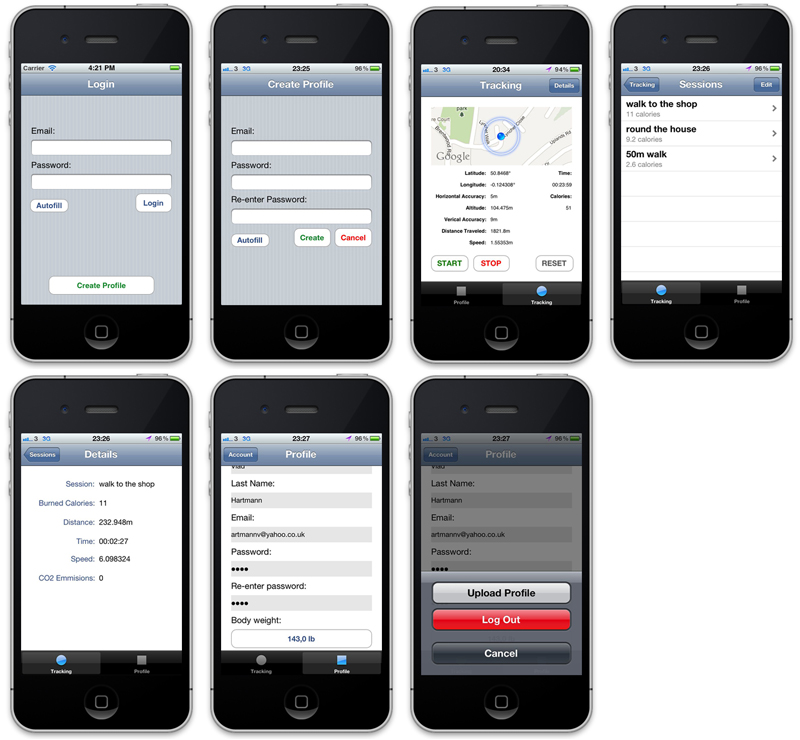
\includegraphics[width=120mm]{/content/PEM-fifthSprintCycle.jpg}
	  \caption{The PEM prototype extended by multi-view functionality.}
	  \label{PEM-fifthSprintCycle}
\end{figure}


\clearpage
\section{Connecting GUI to the application's logic}
In the sixth sprint cycle a main PEM's persistence mechanism and user management were implemented. PEM's requirements specifications state that the application should feature some authentication mechanism. From this point on it became apparent that PEM needed some simple database where profiles could be stored. Each profile would then have sessions (gathered and processed location data and calculations) associated with it.


\begin{figure}[H]
  \centering
	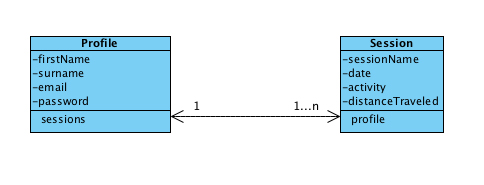
\includegraphics[width=120mm]{/content/PEM-database-Initial.jpg}
	  \caption{PEM's data model with relationships.}
	  \label{PEM-database-Initial}
\end{figure}


This simple data model, when implemented in the Xcode's data modelling tool, worked well. User input validation had to be in place on any text field in the GUI. This was achieved with some simple logic and regular expressions. Linking the GUI to view controllers was explained earlier in the section 'building a simple iPhone application'. It is important to mention at this point that any additional user interface (UI) components added since the simple iPhone application had to also be wired up. Thus appropriate outlets had to be created to output data stored in view controllers' variables into these components.


\clearpage
\section{Creating a profile and logging in}
To use the PEM a user had to log in first. If the user didn't exist they were prompted to create a profile. The way profile creation was achieved was to create a simple profile object with attributes outlined in the Figure~\ref{PEM-database-Initial}. This object then could be stored in a database using Core Data persistence. The detailed procedure would consist of the following:\\ \\
Any iPhone project using a Core Data had to be configured, linking into an appropriate framework and contain specific methods outlined in chosen class e.g. AppDelegate class. These methods then can be delegated to other classes as needed (so no need for a code duplication). A first step to persisting a plain object is to instantiate a Managed Object Context (MOC) by methods from the AppDelegate. A second step is to map the plain object onto Managed Object (MO). The MO is instantiated using an entity description (the data object created earlier in the Xcode's modelling tool) and from the MOC. At this stage there is a MOC containing one MO. Any values from the simple profile object can now be mapped onto the MO. To complete a data persistent procedure a save method is called on the MOC after which the data is stored in a file.\\ \\


\begin{figure}[H]
  \centering
	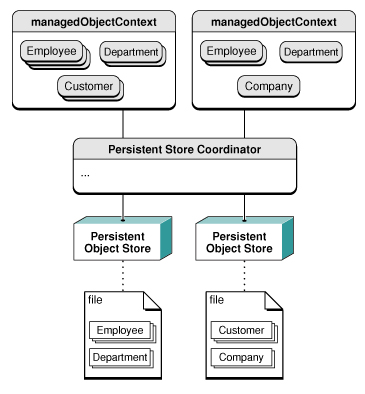
\includegraphics[width=90mm]{/content/AppleCoreData.jpg}
	  \caption{Apple developer website [13]}
\end{figure}


While creating a user profile the user had to only input their email address and two passwords that match, all in a valid format set and verified by regular expressions. The user then could add more details to their profile once logged in. The email address acted as a user name and therefore had to be unique. To achieve uniqueness it was necessary to query a database for any existing data. Querying in a Core Data is called fetching and is done by the following procedure:\\ \\
As before a Managed Object Context (MOC) has to be instantiated. A second step is to instantiate an Entity Description (ED) object providing an object/entity that needs to be fetched and MOC. A third step is to instantiate a Fetch Request (FR) object providing the ED. A fourth step is to instantiate a Predicate (P) object providing a query and value to fetch against and set the predicate to FR. A final step is to instantiate an array by executing MOC's executeFetchRequest method with FR as a parameter and returning any results.
Once the profile was created the user was prompted to login with newly created records.


\section{GPS tracking and creating a session}
A logged user was able to track their position and see a distance travelled. This functionality was implemented by delegating necessary object and method from a Core Location (CL) framework into the tracking view controller. The object involved was called Location Manager (LM). The method responsible for receiving and updating  a user's position had a basic logic, which was later extended. It was discovered that this method was being executed in a loop governed by the LM. It accepted three parameters, all of which were passed in by the CL framework and iPhone GPS hardware. Any functionality inside the method could make use of these parameters. For example, to calculate distance travelled, a starting point was created as soon as a GPS tracking started by assigning a new location to it (only if the starting point was null). CL's method, the distanceFromLocation was called on a new location obtained, passing the starting point as a parameter e.g.\\ \\\textbf{[newLocation distanceFromLocation: startingPoint]}.\\ \\
The location parameters were of a type CLLocation (CoreLocation Location) and supported a number of methods, which could be called to access their attributes. These attributes were for example location coordinates, horizontal or vertical accuracy or speed. For more details please refer to PEMTrackingViewController class in a source code. Any data gathered by the LM were stored in PEMLocationData object on every iteration of the method loop. This way, the PEMLocationData object always contained up-to-date values. It was used for creating a testing data sheet where values could be checked and evaluated or for sharing the values with a rest of the PEM's functionality.\\ \\
The user could pause or stop GPS tracking invoking methods on the Location Manager. When stopping GPS tracking, the user was asked whether to save the data or not. If the user decided to save the data, a PEMsession object was created and all required data from the PEMLocationData object were stored in it (creating a separate PEMSession object rather than reusing the PEMLocationData object was necessary to separate testing and evaluating environment from ready-to-store data). The PEMSession object was then passed to a PEMDataCenter allowing sharing with other view controllers and the view was switched to save session screen. Here a session name could be added, and after pressing a save button, the session was persisted as described in the section Creating a profile and logging in. PEMSession object now updated with a name attribute was stored back into the PEMDataCenter so a sessions view and session details view could use newly saved data.\\ \\
This was an end of the sixth sprint cycle. PEM now was a multi-view application capable of holding multiple users. It could receive and process GPS data and store it as sessions.


\clearpage
\section{Metabolic calculations}
In the seventh sprint cycle it was finally time to implement metabolic calculations, which would produce caloric expenditure. It turned out that there are various ways to do it and all depend on hardware available.\\ \\

\begin{enumerate}
	\item For example, very na\"\i ve caloric expenditure estimations could be done by using caloric expenditure tables and charts. Values in the charts are estimates for a particular activity in a particular time (usually 30 min or 1 hour). All the PEM would need to do is to measure the time of an activity a user performed.\\
	\item A less na\"\i ve method discovered was using walking or running equations as described in Energy Expenditure of Walking and Running, Medicine \& Science in Sport \& Exercise, Cameron et al, Dec. 2004. [14] The walking equation looked like this:\\ \\

\begin{tabular}{ll}
\textbf{C = (W) x (Constant) x (D)}\\ \\
C - Calories burned\\
W - Body weight in pounds\\
Constant - 0.53 (VO$_{2}$/lb/1 mile)\\
D - Distance in miles\\
\end{tabular}\\ \\


	\item Another, more precise way, would be monitoring heartbeats and use them as an input into an equation. For example if the PEM had been constructed in such way that it could process signals (e.g. using the iPhone headphone's microphone to listen to heartbeats on a wrist or neck) an equation exists that can calculate the caloric expenditure [15]:\\ \\


\begin{tabular}{ll}
\textbf{C = (0.6309 x H + 0.09036 x W + 0.2017 x A - 55.0969) x T / 4.184}\\ \\
C - Calories burned\\
H - Average heart rate\\
W - Body weight in pounds\\
A - Person's age\\
T - Length of exercise\\
The decimal values are coefficients derived during development of the equation.
\end{tabular}\\ \\


It has been decided however that processing the signals in the PEM would be too hard to implement in a time given.\\ \\


	\item In research by Simon Hay, Stamatina Th. Rassia , Alastair Beresford and Nick V. Baker \textsf{'}Movement dynamics in office environment' has been shown that when a person accelerates, they must gain kinetic energy [16]. Their energy expenditure model was expressed as:


\begin{figure}[H]
  \centering
	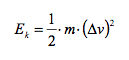
\includegraphics[width=40mm]{/content/KineticEnergy.jpg}
\end{figure}


\begin{tabular}{ll}
Ek - energy expenditure in J\\
m  - mass in kg\\
\ensuremath \Delta v - change in velocity in m/s\\
\end{tabular}\\ \\


 \item While carrying out research of this approach it turned out that there is a relationship between the Kinetic Energy and Work [17]. Therefore there is yet another way to estimate energy expenditure [18]:\\

\end{enumerate}

\begin{tabular}{ll}
\textbf{Wj = Fn x Dm}\\ \\
W - work in joules\\
F - force in newtons = mass x acceleration\\
D - distance in meters\\
\end{tabular}\\ \\


None of the methods discovered were suitable for the desired outcome of PEM and its use of GPS data. Either they have been very trivial or needed to utilise the iPhone's accelerometer hardware. While further research of available methods was under way, it has been decided to implement the Cameron's walking equation for testing purposes.

\clearpage
\subsection{ACSM MetCalcs}
A few days later, a book released by American College of Sport Medicine (ACSM), the ACSM's Metabolic Calculations Handbook, was discovered which featured new ways of calculating caloric expenditure. Attention focused towards these ideas as they were deemed the best solution so far.
\\ \\
The ACSM MetCalcs were introduced in 1975 in a publication known as \textit{Guidelines for Exercise Testing and Prescription (GETP)}. It is a set of equations gathered by several authors over years from many scientific publications. The book emphasizes estimating the energy consumption by calculating values of oxygen in nonclinical environments without the need for specialised and expensive hardware.

\subsubsection{Exercise science prediction}
In the exercise science prediction, it is often preferred to estimate a value rather than directly measuring it. This is for various reasons, such as time it takes to perform the measurement, expense of hardware involved or the inconvenience caused to the client while performing the measurement.

\subsubsection{Metabolic primer}
"Energy requirements can be expressed in terms of the oxygen requirements of the physical activity being performed - commonly referred to as the oxygen consumption or oxygen cost (VO$_{2}$)" [19]. VO$_{2}$ is best known as a maximal measure (VO$_{2 max}$) and provides useful information in area of cardiorespiratory fitness. The best possible way to measure VO$_{2}$ of a physical activity is using the open-circuit spirometry. "The term, open-circuit spirometry, refers to the method of conducting spirometry where the subject takes a maximal inspiration from the room, inserts the mouthpiece into the mouth, and then blows out either slowly (SVC) or rapidly (FVC) until the end-of-test criterion is met" [20]. As already mentioned, this technique is difficult to carry out in many health or fitness settings and that is why the ACSM MetCalcs became popular between health and fitness practitioners.

\subsubsection{Expression of energy use}
All actions in human body need or use energy for example for digestion of food or for muscle contraction. This is called metabolism and it is all about energy use or energy production. Energy or oxygen use can be expressed in many ways by following terms:\\
\begin{enumerate}
	\item \textbf{Metabolism} - function of time and intensity.
	\item \textbf{Exercise metabolism} - energy expenditure.
	\item \textbf{Aerobic metabolism} - production of energy using oxygen.
	\item \textbf{Oxygen consumption} - amount of oxygen (VO$_{2}$) consumed typically as rate or per minute.
	\item \textbf{Relative oxygen consumption} - oxygen consumption relative to body weight, expressed in mL/kg/min.
	\item \textbf{Absolute oxygen consumption} - oxygen consumed by the person per unit of time expressed in litres per minute. It is useful because it allows for easy estimation of caloric expenditure (one liter of O2 is associated with burning of 5 kcal).
	\item \textbf{Gross VO$_{2}$} - total oxygen consumption.
	\item \textbf{Net VO$_{2}$} - oxygen consumption of activity only.
	\item \textbf{VO$_{2rest}$} - the resting component. Value of oxygen expended at rest is estimated at 3.5 mL/kg/min.
\item \textbf{Calories} - expression of energy intake and expenditure commonly used to quantify the amount of energy derived from food. A calorie is a very small unit and therefore kcal is used in calculations of human energy expenditure instead. One kcal equals 1000 calories. However, conventionally it is most of the time found that terms Calories or calories are used interchangeably on packaging, which means the same as kcal. The small calorie unit is used only for scientific purposes.\\ \\
\end{enumerate}


The ACSM MetCalcs include five equations to estimate energy expenditure. The walking, running, leg ergometer (cycling), arm ergometer and stepping. With time available to implement the PEM only the walking and running equations were selected for the calorie expenditure model.\\ \\

\clearpage
\subsubsection{ACSM Walking equation}
The ACSM's walking equation can be used for estimating caloric expenditure during walking activities. There are three components within the walking equation. Each of these components represents aspect of energy expenditure.

\begin{enumerate}
	\item Oxygen cost of moving one kilogram of body weight one meter. This has been estimated to be 0.1 mL/kg/m. The Horizontal Component of walking can be therefore computed as:\\

\textbf{Horizontal Component = Speed (m/min) x 0.1 mL/kg/m}\\
	
	\item To compute the Vertical Component of walking we need to know:
	\begin{enumerate}
		\item The oxygen cost of moving vertically against gravity. This has been estimated to be 1.8 mL/min/m.
		\item The rate of the movement (speed)
		\item The steepness of the vertical climb (grade)\\
	\end{enumerate}


This can be re-written as:\\

\textbf{Vertical Component = Speed (m/min) x Grade (decimal) x 1.8 mL/min/m}

\subsubsection{Computing Grade}
"Vertical ascent is denoted by grade, typically calculated as a fraction (decimal) and then converted to percent. Percent grade reflects the degree of elevation gain for give horizontal distance."\\

Example:\\

A rise of 1 m over distance of 10 m \\ =
1 m / 10 m \\ = 0.10 \\
0.10 x 100 - 10\% grade\\


	\item The Horizontal and the Vertical components represent together the net oxygen cost of walking (walking Net VO$_{2}$). To obtain the gross oxygen cost of walking (walking Gross VO$_{2}$) we must add in the resting component (VO$_{2}$rest).
\end{enumerate}
To put it all together the ACSM walking equation is:\\ \\
\textbf{VO$_{2}$ (mL/kg/min) = [Speed (m/min) x 0.1 mL/kg/m] +
          [Speed (m/min) x Grade (decimal) x 1.8 mL/min/m] +
          3.5 mL/kg/min}\\


\subsubsection{Limitations of the Walking Equation}
Results of the walking equation can only be accurate when an activity being performed is a steady-state activity. If the activity is non-steady, for example in the last stage of maximal exercise set, the equation will produce inaccurate results. The equation accuracy is also dependent upon a speed range between 1.9 - 3.7 miles per hour. Above the given speed range, walking economy changes and a person of a particular height may run instead.\\ \\


\clearpage
\subsubsection{ACSM Running equation}
The ACSM's running equation is similar to the Walking Equation except that for running the Horizontal Component requires twice the oxygen. The Vertical Component is also different.\\ \\
The ACSM running equation is:\\ \\
\textbf{VO$_{2}$ (mL/kg/min) = [Speed (m/min) x 0.2 mL/kg/m] +
          [Speed (m/min) x Grade (decimal) x 0.9 mL/min/m] +
          3.5 mL/kg/min}

\subsubsection{Limitations of the Running Equation}
As with the walking equation results of the running equation are only valid for steady-state activity. Speed must be greater than 5.0 miles per hour.\\

\clearpage
\subsubsection{Determining the oxygen cost and caloric expenditure}
We can compute caloric cost if we know the absolute VO$_{2}$ in L/min.\\ \\
Example:\\ \\
Step 1. Determine the oxygen cost of walking activity.\\ \\
Speed = 2.9 miles per hour x 26.8 = 77.72 meters per minute\\
Grade = 2 \% / 100 = 0.02\\ \\
VO$_{2}$ (mL/kg/min) = [77.72 (m/min) x 0.1 mL/kg/m] +
          [77.72 (m/min) x 0.02 x 1.8 mL/min/m] +
          		         3.5 mL/kg/min
		      = 7.77  + 2.80 + 3.5
		      = 14.07 mL/kg/min\\ \\
Step 2. Convert VO$_{2}$ in mL/kg/min into VO$_{2}$ in mL/min. We need to multiply by body weight.\\ \\
VO$_{2}$ (mL/kg/min) x BW\\
= 14.07 x 65\\
= 914.55 mL/min\\ \\
Step 3. Convert VO$_{2}$ in mL/min into VO$_{2}$ in L/min. We need to divide by 1000.\\ \\
VO$_{2}$ (mL/min) /1000\\
= 914.55 / 1000\\
= 0.91 L/min\\ \\
Step 4. Convert VO$_{2}$ in L/min into kcal/min. We need to multiply VO$_{2}$ (L/min) by 5.\\ \\
VO$_{2}$ (L/min) x 5\\
= 0.91 x 5\\
= 4.55 kcal/min expended\\


\clearpage
\subsubsection{ACSM MetCalcs Prediction Error and Limitations}
When estimations and predictions are being made, we should be willing to understand and accept some amount of error. The most common expression of prediction error is the standard error of estimate (S.E.E). Thus, even though the measured VO$_{2}$ at the same exercise intensity for the same individual will be very similar, it could have the S.E.E of up to 7\% for 69\% of individuals. Therefore the equations work well if tracking the same individual over time rather than comparing the VO$_{2}$ between different subjects.\\ \\
As previously mentioned, the equations presuppose that the activity is a steady-state one and the correct equation is used in accordance with correct speed of activity.
The accuracy of equations is not affected by most environmental influences such as heat or cold but mechanical variables such as gait abnormalities, wind, snow or sand will contribute to inaccurate results.\\


\clearpage
\section{Implementing ACSM MetCalcs into PEM}
Once knowledge ACSM's metabolic calculations had been acquired it had to be implemented into PEM. A class PEMMetabolicCalculations was created which held methods to calculate walking and running VO$_{2}$ as previously explained. These methods took one parameter, the PEMLocationData object containing values gathered during GPS tracking, and were executed in set intervals from the PEMTrackingViewController. The values had to be converted into appropriate units. The methods returned computed VO$_{2}$ values, which served as an input to the calorie expenditure method.


\begin{figure}[H]
  \centering
	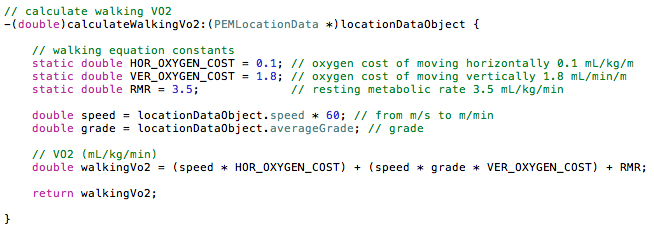
\includegraphics[width=120mm]{/content/CalculatingVO2code.jpg}
	  \caption{PEM's code snippet for calculating VO$_{2}$ of walking activity}
\end{figure}


\begin{figure}[H]
  \centering
	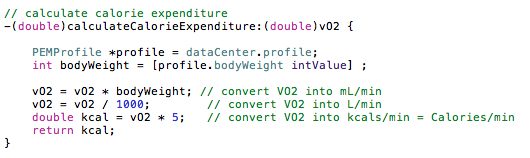
\includegraphics[width=120mm]{/content/calculatingCaloriesCode.jpg}
	  \caption{PEM's code snippet for calculating caloric expenditure}
\end{figure}

\clearpage
It is important to mention here the development stage where a grade had to be computed. 
It is know that the grade value needed as an input to both metabolic equations can be computed by:\\
\begin{enumerate}
	\item Obtaining one position point and its altitude
	\item Travel some distance
	\item Take another position point with altitude
	\item Measure a distance between these two points
	\item Subtract the altitude of the first position point from the second one to get a rise
	\item Divide rise by distance\\
\end{enumerate}


\begin{figure}[H]
  \centering
	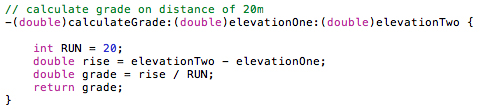
\includegraphics[width=120mm]{/content/calculateGradeCode.jpg}
	  \caption{PEM's code snippet for calculating grade}
\end{figure}


A problem, however, was that results of the grade computation were extremely inaccurate when using an altitude produced by iPhone's Core Location framework (as outlined in section Utilizing Apple's Core Data and Core Location). For this reason, the Google Elevation API was used to obtain accurate altitude.
\\ \\
The Google Elevation API (GEAPI) is a REST web service, which provides accurate altitude data. GEAPI is free to use and devices or other software make use of it by sending GET requests to it with latitude and longitude coordinates. The web service responds with the altitude value. The response is formatted either in XML or JSON.\\ \\
The REST web service is a software system that provides functionality of some other software system, for example weather applications, over the Internet. The weather application (also referred to as a server) could be written in a particular programming language like Java and therefore could be accessed over the Internet only by other Java applications called clients. A purpose of the web service is to create an intermediate point of access between the client and the weather application. The REST web service is written in such a way that clients written in various languages can communicate with it by simple commands known as HTTP verbs (GET, POST, UPDATE, DELETE). This way, if a client written in, for example, Objective-C programming language wants to know what the weather is, it sends a simple GET request to the web service, which then contacts the weather application and returns weather data back to the client.
The XML stands for eXtensible Markup Language and it has been designed to transport and store data.


\begin{figure}[H]
  \centering
	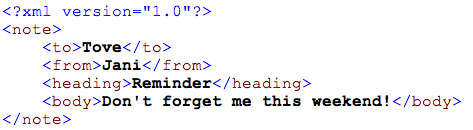
\includegraphics[width=120mm]{/content/XMLcode.jpg}
	  \caption{An example of a XML file}
\end{figure}


The JSON stands for JavaScript Object Notation and is a lightweight data-interchange format, based on the JavaScript programming language. It is easy to read and write for humans and easy for machines to generate and parse. JSON is an independent programming language but uses conventions of the C-family of programming languages. A JSON file is built from a collection of name/value pairs (hash table, keyed list) and an ordered list of values (array, vector, list).


\begin{figure}[H]
  \centering
	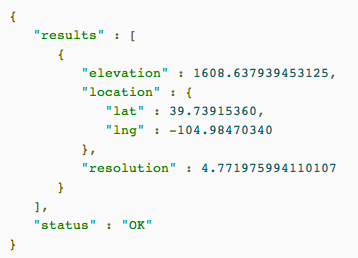
\includegraphics[width=120mm]{/content/JSONfile.jpg}
	  \caption{An example of a JSON file}
\end{figure}


To make use of the Google Elevation API web service (server) the PEM (client) had to be able to communicate with it and receive data from it. Communication had a form of sending a simple GET request to the server to which server responded by sending requested data. To send and receive data between client and server over a network following had to be done:\\

\begin{enumerate}
	\item Send data to a web service
	\begin{enumerate}
		\item Data from the client (object with variables holding the data) had to be parsed into interchangeable JSON format
		\item The interchangeable JSON data then had to be serialised (converted into array or bytes which could be carried over the network)
		\item Send data to the web service\\
	\end{enumerate}

	\item Receive data from a web service
	\begin{enumerate}
		\item De-serialize received data
		\item Map the data in JSON format onto PEM's object\\
	\end{enumerate}
\end{enumerate}

Because this procedure is very repetitive, and can introduce parsing errors the RestKit framework has been used instead.\\ \\


RestKit is an Objective-C framework for iOS that makes interacting with REST web services simple and fast. It combines a HTTP request/response API with an object mapping system. This reduces the amount of code developers need to write so they can focus more on their data model and worry less about the details of sending requests, parsing responses, and building representations of remote resources.
An unexpected behaviour started to appear in form of a null pointer exception when attempting to receive data from GEAPI. After thorough debugging, it has been found that while waiting for data to arrive from the web service, a method processing the data has been executed many times already with zero altitude. The reason for this was the asynchronous data transfer used by the RestKit framework. The asynchronous data transfer is a conventional way of sending and receiving data in a background while the application is running so the GUI can remain responsive to the user. By running in the background, it is meant to run in a separate thread of execution while GUI runs in a main thread and the user can still interact with it. If the synchronous data transfer would be used, functionality dealing with transferring data would be most likely running in the same thread as GUI, which would become frozen until the data transfer is complete. A concept of asynchronous method execution is well know and there are many ways of how to deal with it. In Objective-C language, the best know way is to use the notification system, also known as event handling in other programming languages, where a given method executes only if other method notifies it. The notification only takes place if some event happens, in our case, if data is received. The theory of this concept was understood but due to time constrains it could not be implemented. Instead, an iterative execution of a method that prints a word "Receiving…" was put in place to postpone further execution of code until data is received.\\ \\
With accurate altitude data received from the GEAPI and mapped onto PEMLocationData object, the PEM could use it its metabolic calculations.


\clearpage
\section{Carbon footprint calculations}
When searching for ways to calculate carbon footprint of individuals, the vast majority of information sources provided ready to use CO$_{2}$ emission calculators or energy conversion factor tables. The reason for this is that performing manual calculation is difficult due to huge variations in regional areas, CO$_{2}$ emissions from different types of vehicles and each information source saying varying amounts. The Carbon Trust website [21] seemed as a reliable and up-to-date source of information with estimate data of carbon footprint for individuals using a particular mode of transport.\\ \\
Implementing the CO$_{2}$ emission calculations into PEM was not difficult. All that was needed was a distance and value estimate for the mode of transport from the Carbon Trust energy conversion factor table. There were three methods for calculating carbon footprint for three modes of transport the Car, Bus and Train. The following snippet of code shows the calculation for estimating CO$_{2}$ emissions of PEM's user traveling by train.


\begin{figure}[H]
  \centering
	\includegraphics[width=120mm]{/content/CO2CalcsTrain.jpg}
	  \caption{PEM's code snippet calculating CO$_{2}$ emissions of user traveling by train}
\end{figure}


Again, as with metabolic calculations, methods to calculate CO$_{2}$ emissions were invoked in intervals from the PEMTrackingViewController to give real-time data.
The user of PEM, even though traveling and not performing any physical activity, was still expending energy and therefore notified about their VO$_{2}$rest and caloric expenditure.\\ \\


\clearpage
\section{Implementing the PEMWEBAPP}
The aim of the eighth sprint cycle was to build a web application (PEMWEBAPP) that the PEM could send a data to. This web application would store received data in its local database and present it to user once they would log in. At early stages of developing the PEM, it was not completely decided how the web application should be built. However, knowledge about building websites and utilising a network socket communication (interfaces that can plug into each other to allow programs communicate over the network) from the past suggested that the PEMWEBAPP could be built.\\ \\
When development of PEM was in the final stages, an introduction into course module Web Applications and Services opened the door to another solution of how to build the PEMWEBAPP. It turned out that accessing the PEMWEBAPP's database through a socket directly from the PEM could introduce a potential security risk. Utilising knowledge obtained form the Web Applications and Services module, implementation of the desired web application could begin step by step in a correct way.
One of the first steps in building a PEMWEBAPP was to set the appropriate environment for web development. MySQL database, Eclipse IDE and Glassfish have been installed and configured. The Eclipse is an Interactive Development Environment, where application coding is being done. The Glassfish is an open-source application server, developed by Oracle. The application server is software that provides the environment for running web applications. This environment supports many features such as database connectors, web server, transaction manager, security system and many more. Database connectors are needed to create bridges between a web application and database. There is many different vendors of database systems, therefore there must be a connection mechanism for each of them.  Glassfish supports the vast majority of connectors, including MySQL. A web server is software that serves web pages when a request arrives from a client (web browser).  A transaction manager is software that manages transactions in the application server. A transaction is a sequence of steps that must be executed to arrive at a desired result. In the remote environment, for example when modifying data on a Facebook profile, a sequence of steps must be performed (establish connection with database, change content of data, save data and notify user).  If at any point during the execution of the steps an error occurred, e.g. no Internet connection, the transaction is rolled back and data stays unchanged. The security system of an application server makes it easy to secure a web application by supporting different security realms or role managements.\\ \\
With this configuration running locally on a computer used for development (localhost) the implementation of PEMWEBAPP could start. However, to test data transfer from PEM to PEMWEBAPP over a network, a remote deployment environment had to be set up as well. The initial idea was to rent a remote virtual server from a hosting company and perform all necessary setups as for localhost. This worked well except that the cost associated with renting the server was unnecessary. After some research and with help of howtoforge.com [22] a home server was set up on old desktop computer. The WMware's EXSi hypervisor was installed first. A hypervisor is a virtual machine manager used as one of many hardware virtualisation techniques. ESXi is installed directly on a physical hardware of the computer and partitions it into multiple virtual machines that can run simultaneously, sharing the physical resources of the underlying computer. Once partitioned, the Ubuntu server was installed on one of the partitions. The Ubuntu server is a Linux server and is free. The idea of making a virtualisation was due to the need to install other servers (such as windows server) in future on a single computer. One important part of this remote deployment setup was to configure the home Internet router. The home server needed to be accessible from the Internet outside of the house not just in the local network at home. This was achieved by setting a port forwarding on a router. The port is a communication channel, which can be assigned to any program running on the computer so it can accept communication from the network. Programs such as Glassfish or MySQL database have their ports and other programs can communicate with them using these ports. A standard router setup does not provide access to any port from outside the Internet for security reasons so this had to be configured in a router's port forwarding table. Once configured, a request to access a particular program or resource on the home server can arrive from outside the Internet to the home router. From here it is channelled via a particular port to the program or resource.

\subsubsection{Java EE}
The process of developing the web application started by learning about Java Enterprise Edition (JavaEE). JavaEE is a standard set of libraries enabling a programmer to write a server side code. The word standard means that the libraries are compatible with lots of application servers from different vendors such as Oracle, IBM, Red Hat, Adobe, etc.

\subsubsection{Enterprise Java Beans}
Creating a java web application is very similar to creating a standard java application. The only difference is that java classes of web applications must have some additional annotation in them to be executable in the application server. By providing this annotation, a basic java class becomes an Enterprise Java Bean (EJB). This EJB now has also additional features such as: its methods become transactional, secure and remote and class becomes to have an easy database integration. The PEMWEBAPP has four EJB's. Two for dealing with communication from PEM and two for dealing with communication from a web browser. The IphoneDataAccessImplementation and DataAccessImplementation are both dealing with accessing PEMWEBAPP's database. They are called Data Access Objects (DAOs). On top of the DAOs, there are the remaining two EJBs, the IphoneDataManipulationImplementation and DataManipulationImplementation. These act as data manipulation classes. Because the PEMWEBAPP has nearly no business logic, these classes act only as delegates. If the application was to be extended in future, this is the place for further functionality.


\subsubsection{Java Persistence and Entity Beans}
There are two main libraries to access database in Java. The Java Database Connectivity (JDBC) and the Java Persistence API (JPA). The JDBC is a mechanism that allows a programmer to issue SQL statements to any database that supports Java. The SQL or Structured Query Language is a programming language for managing data in relational database management systems. JDBC is suitable for some purposes, but it is very low level and requires significant amount of code to be written to transfer rows of data in a database into collections of java objects. On the other hand, the JPA allows the programmer to work with regular java objects, and with simple annotations in classes of those objects, it will create automatically the SQL needed. Such annotated classes are called Entity Beans (EB) because they represent an entity in relational database. In a code snippet below we can see different annotations for various JPA actions such as for setting up unique, auto incrementing id of entity of setting up one-to-many relationship with any changes to be cascaded to related entity.


\begin{figure}[H]
  \centering
	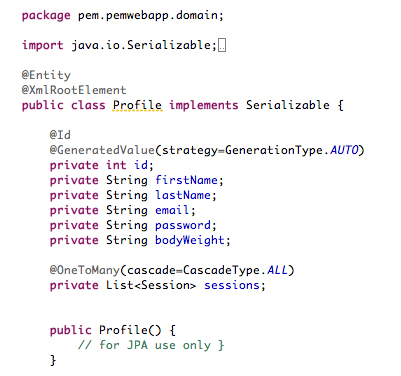
\includegraphics[width=120mm]{/content/EntityBean.jpg}
	  \caption{The Entity Bean which creates an object from regular Java class and stores it in a database}
\end{figure}


\subsubsection{JSF}
To write a dynamic web pages in Java (web pages that change content all the time) there are libraries such as Servlet and JSP APIs that can be used. Both are however very dated and any serious work requires tedious coding, as they are low level. A newer and more elegant solution is to use Java Server Faces (JSF), which allows a programmer to build dynamic web pages at higher level of abstraction. Instead of, for example, building HTML tables, JSF works using components. The components consist of a regular HTML and can be anything from charts, trees or buttons to image galleries.\\
To create a web page that uses JSF components we use XHTML file. XHTML stands for EXtensible HyperText Markup Language and is almost identical to HTML but it is stricter and cleaner. We need to import the JSF components library into that file by declaring an import statement at the top of the file. 
JSF is a basic components library built into JavaEE. There are many third party components libraries available and one of the most popular and free is the PrimeFaces. PrimeFaces is an open source JSF component suite with various extensions and Ajax support. The Ajax support makes PrimeFaces very advance component library and enhances user experience. Ajax stands for asynchronous JavaScript and XML. The power of this technology is in exchanging data with a server, and updating parts of a web page, without reloading the whole page.\\ \\
JSF components are well configurable to fit with web page design. The figure~\ref{JSFpageStat} below shows a statistics page from the PEMWEBAPP, where a line chart component pulls caloric values from a PEMWEBAPP's database.


\begin{figure}[H]
  \centering
	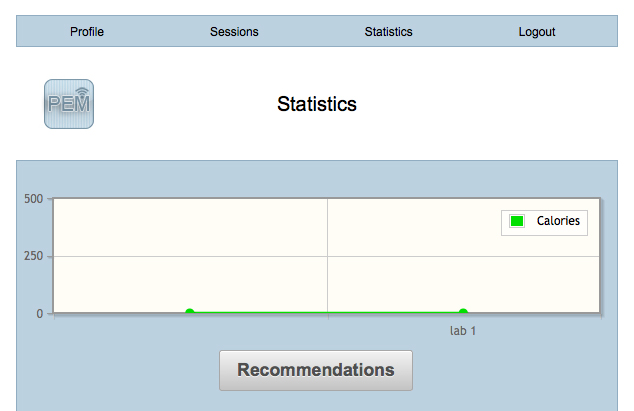
\includegraphics[width=120mm]{/content/JSFpageStats.jpg}
	  \caption{The JSF page using PrimeFaces chart component displayed in a web browser}
	  \label{JSFpageStat}
\end{figure}


\subsubsection{Backing Bean}
Having a nice looking JSF web page is only one part of story. To make a web page dynamic we need some way of accessing a logic written in a java class. Again, as with EJB, a basic java class can be annotated to act as a Backing Bean (BB) for a web page. This backing bean will contain any required functionality and will be connected to the XHTML file created earlier. The following code snippet in figure~\ref{BackingBean} is from a Profile Backing Bean and shows some basic functionality that particular dynamic page needs. PEMWEBAPP has four Backing Beans, one for each page.


\begin{figure}[H]
  \centering
	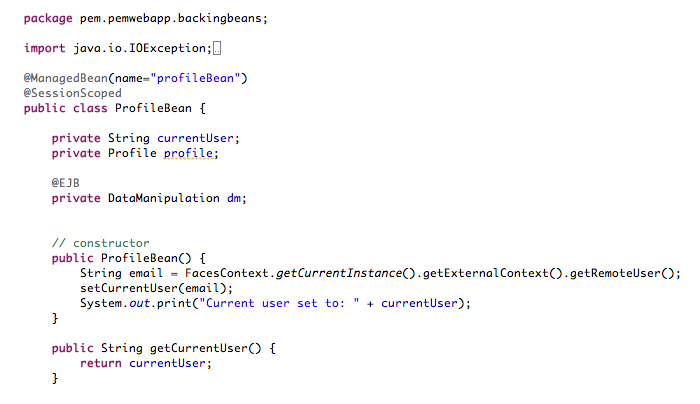
\includegraphics[width=120mm]{/content/BackingBean.jpg}
	  \caption{Code snippet of the PEMWEBAPP Profile's Backing Bean}
	  \label{BackingBean}
\end{figure}


\subsubsection{Expression Language}
To connect the backing bean to the XHTML file, we use the Expression Language (EL). EL, also known as Unified Expression Language, is a special purpose programming language mostly used in Java web applications. It is used for embedding expressions into web pages. EL was developed by Java specification writers but can be used for a variety of technologies. The following snippet of code in the figure~\ref{EL} shows connecting a web page to its backing bean. More specifically a line chart component accessing data from database through a Backing Bean.


\begin{figure}[H]
  \centering
	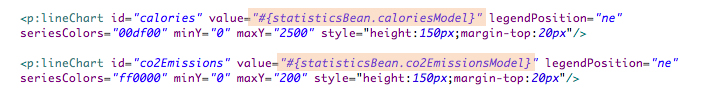
\includegraphics[width=120mm]{/content/EL.jpg}
	  \caption{Code snippet of the EL embedded in JSF component's tag}
	  \label{EL}
\end{figure}


\subsubsection{Dependency injection}
On many ocassions in web development, there is a need for intercommunication between BB and EJB. To access EJB functionality in a BB we use a dependency injection. "A dependency injection is a software design pattern that allows a choice of components to be made at run-time rather than compile time." [23]. We can inject the Enterprise Java Bean to the Backing Bean by declaring the EJB as a variable in BB with appropriate notation. Because a database access in the PEMWEBAPP is handled by EJB, it had to be injected into our Backing Bean.


\subsubsection{Creating a REST web service}
It has already been described what a REST web service is. To implement one in JavaEE we use a Java API for REST web services (JAX-RS) library and yet more annotations. The REST is built on a concept of resources. As we know the PEM will need to create or access a profile on the PEMWEBAPP. So we need to create a resource representing the profile. This is done by creating a Java class in which we describe a list of operations that we want to expose to a client, in our case the PEM. It is not important how we call these methods because client will not call them directly. The client will make a GET request with specific user i.d. (in our case email) instead, which will be routed to a particular method annotated by the @GET annotation. We also need a URL for this method so the client will find it. The following snippet in the figure~\ref{restWebService} shows the required annotations for creating a REST web service.\\ \\


\begin{figure}[H]
  \centering
	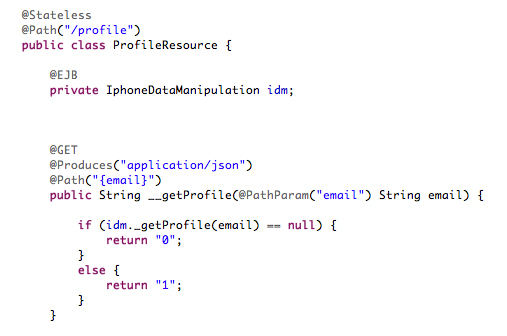
\includegraphics[width=120mm]{/content/restWebService.jpg}
	  \caption{Code snippet for creating a REST web service}
	  \label{restWebService}
\end{figure}


First, a default path above the class declaration is set to represent a root. Then a specific point of access is set above the appropriate method. As PEM's GET request with a specific email address arrives to method, the email address is extracted from the request and used as a parameter in that method. The method then calls appropriate logic and returns results back to the client. The annotation "$@$Produces" tells JAX-RS to parse the results into a specific format, in our case the JSON.

\subsubsection{Securing the PEMWEBAPP}
It has already been mentioned that our application server, the Glassfish, provides functionality to secure any web applications running in it. This is done by configuring an application's web.xml file. The web.xml file is a configuration file that every java web application must have to be deployed onto the application server. A setting, such as those for configuring a REST web service or an application's security, are configured here. The security of the PEMWEBAPP is set up to use user authentication with a JDBC Realm. A JDBC Realm is a way of securing a web application using a database. What this means is that a user's login and password are stored in a database and encrypted. When a user enters their credentials into a login page when logging into the PEMWEBAPP, a Glassfish mechanism compares these with details stored in PEMWEBAPP's database.
We could go as far as securing the REST web service by specifying access to individual users accessing individual methods if we wanted to. In fact, the PEMWEBAPP's web service is currently open to any client with no authentication required. Data transfer between PEM and PEMWEBAPP is also not secured and data are crossing a network without being encrypted. This can cause a potential risk of data being eavesdropped or the web service being accessed by anyone. Both features however could not be implemented due to time constraints.


\begin{figure}[H]
  \centering
	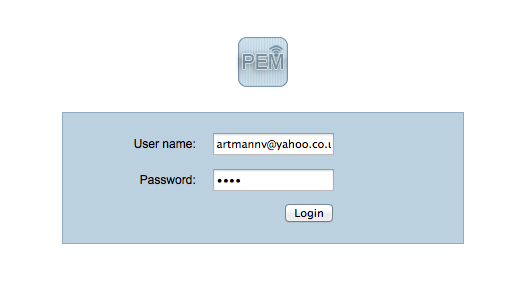
\includegraphics[width=120mm]{/content/PEMauthentication.jpg}
	  \caption{PEMWEBAPP's user authentication page}
\end{figure}


\subsubsection{Completion of PEM and PEMWEBAPP}
In the ninth sprint cycle PEM's profile upload feature was implemented as well as any final design changes to the GUI in resulting both applications being complete.\\ \\
The profile upload feature included nearly all iPhone development techniques learned at this point and was considered hardest to implement. It included:\\
\begin{enumerate}
	\item Extensive use of RestKit and it's powerful object mapping
	\item Pulling data from Core Data
	\item Intercommunication between view controllers
	\item And updating GUI\\
\end{enumerate}
It has been briefly mentioned already that RestKit uses object mapping to send and receive data to and from a web service. But to really understand what is going on, here are the steps involved:

\begin{enumerate}
	\item Set a transfer manager with root URL for the web service to be accessed
    \item Define a default resource path for the HTTP verbs (GET, POST, PUT, DELETE)    
    \item Define mapping of all reqired objects to be transferred. Note that we can map also all necessary realtionships. In our case the Profile can have many Sessions.
	\item Set up a serialisation machanism. In our case we want to serialise JSON objects to byte of array when sending the data to server and de-serialising from byte data to a JSON file when receiving the data from the server.
    \item Register the mapping with the transfer manager
	\item Send or receive the data to or from the web service\\
\end{enumerate}
One of the downsides of the profile upload feature is that it does not support update. This would involve data synchronisation between both PEM and PEMWEBAPP because the user of the web application can delete the profile online. Conceptually it is not hard to design. All that is needed is to send a GET request from PEM to PEMWEBAPP and get back a current state of user's profile. Any attempts to program this functionality however have been unsuccessful due to limited knowledge of the RestKit framework. What is happening instead, is that all stored data in PEMWEBAPP's database are being replaced with those from PEM on every POST request. This way the user always sees the same data in PEMWEBAPP as they are in the PEM.


\subsubsection{Finishing the PEM's GUI}
One of the last changes in the PEM's user interface was to add an activity screen where the user chooses the activity being monitored and recommendation popup windows. Recommendation windows are being populated with relevant content depending on a type of activity being monitored. For example, if a user saves a session of walking activity, the recommendations will advise them on important facts about recommended daily caloric intake or what to do to lose or maintain weight. If a user on the other hand saves a session of traveling by car, they will be advised about planetary wellbeing and top tips on how to reduce CO$_{2}$ emissions.


\begin{figure}[H]
  \centering
	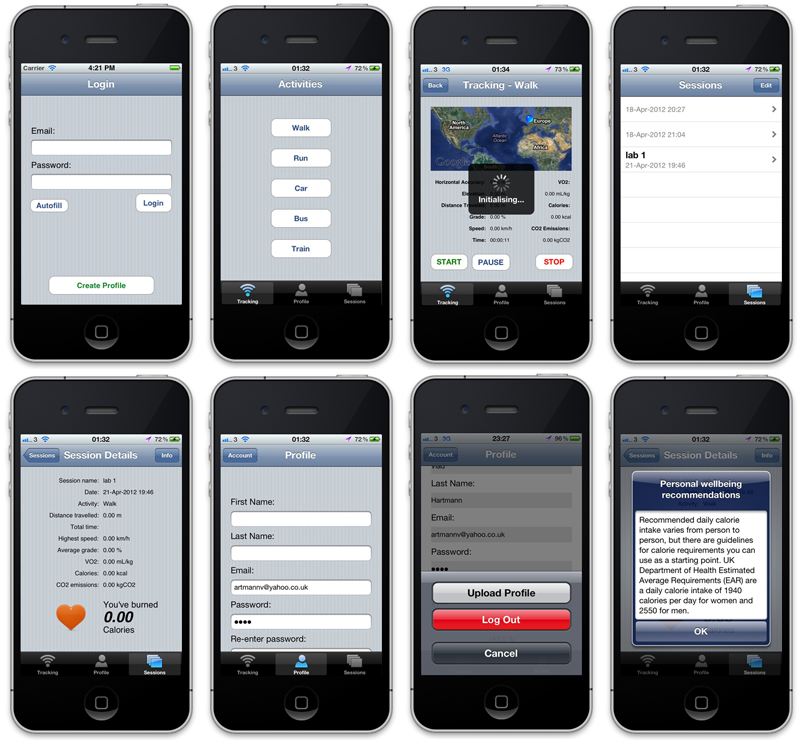
\includegraphics[width=120mm]{/content/PEMfinished.jpg}
	  \caption{Completed PEM application}
\end{figure}


\clearpage
\section{Maintenance and scalability}
It was difficult to pinpoint the exact stage for a solid design, however, when the applications started to grow and there was a potential for scalability and maintainability, further development was becoming difficult to manage. Bearing in mind possible changes to the systems in future, the object-oriented design (OOD) seemed the most appropriate. Because OOD supports modularity, independent objects can be easily changed without affecting overall system. The following are the steps (as described by Ian Sommerville [24]) used in developing both PEM and PEMWEBAPP applications.


\subsection{Understanding and defining the context}
	
	
\begin{figure}[H]
  \centering
	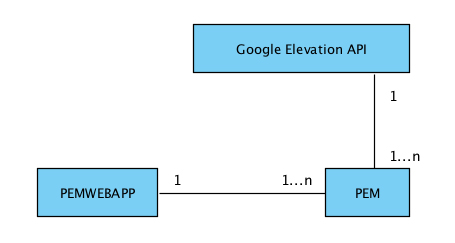
\includegraphics[width=120mm]{/content/PEMcontextDiagram.jpg}
	  \caption{Context diagram showing interaction between PEM, PEMWEBAPP and Google Elevation API third party system}
\end{figure}


\subsection{Designing systems architecture}
To better understand how PEM and PEMWEBAPP applications should be organised, architectural design phase has been used with focus on a design view of the applications. The design view includes architectural patterns, which are outlined below. This level of abstraction allowed both programs to be decomposed into individual components. The only correct way of developing iPhone applications is to follow a Model-View-Controller (MVC) architectural pattern, thus development of the PEM application shall be following it.\\
	

\begin{figure}[H]
  \centering
	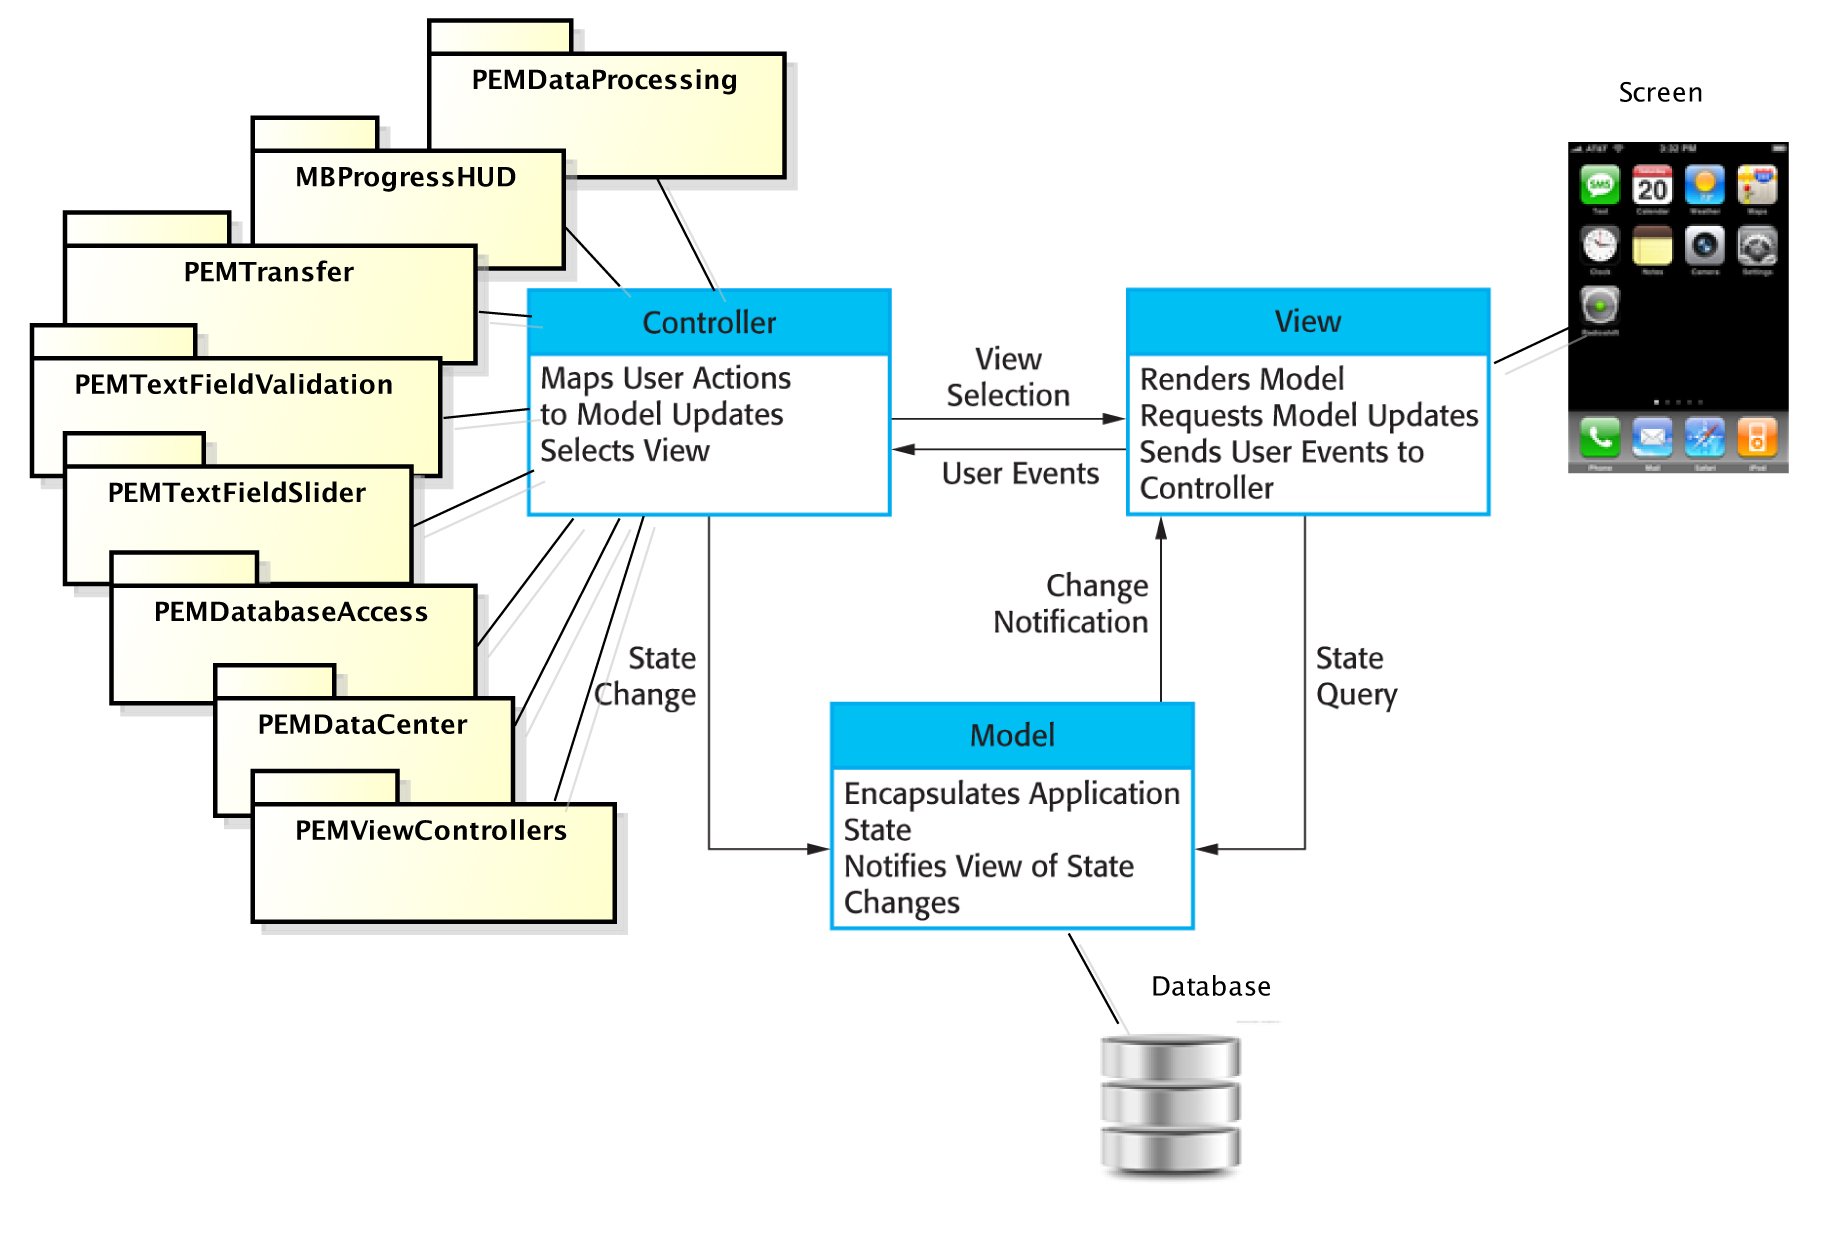
\includegraphics[width=120mm]{/content/MVC-withPackages.jpg}
	  \caption{PEM MVC. Diagram originates from [25] and has been improved to reflect PEM's architecture.}
\end{figure}


Although the PEMWEBAPP application will be deployed on a desktop computer rather than an iPhone, it has similar properties to PEM and therefore using the MVC pattern would also be a good choice. However for experimental purposes, the layered architectural pattern has been chosen instead as it is another way of achieving separation and independence.\\


\begin{figure}[H]
  \centering
	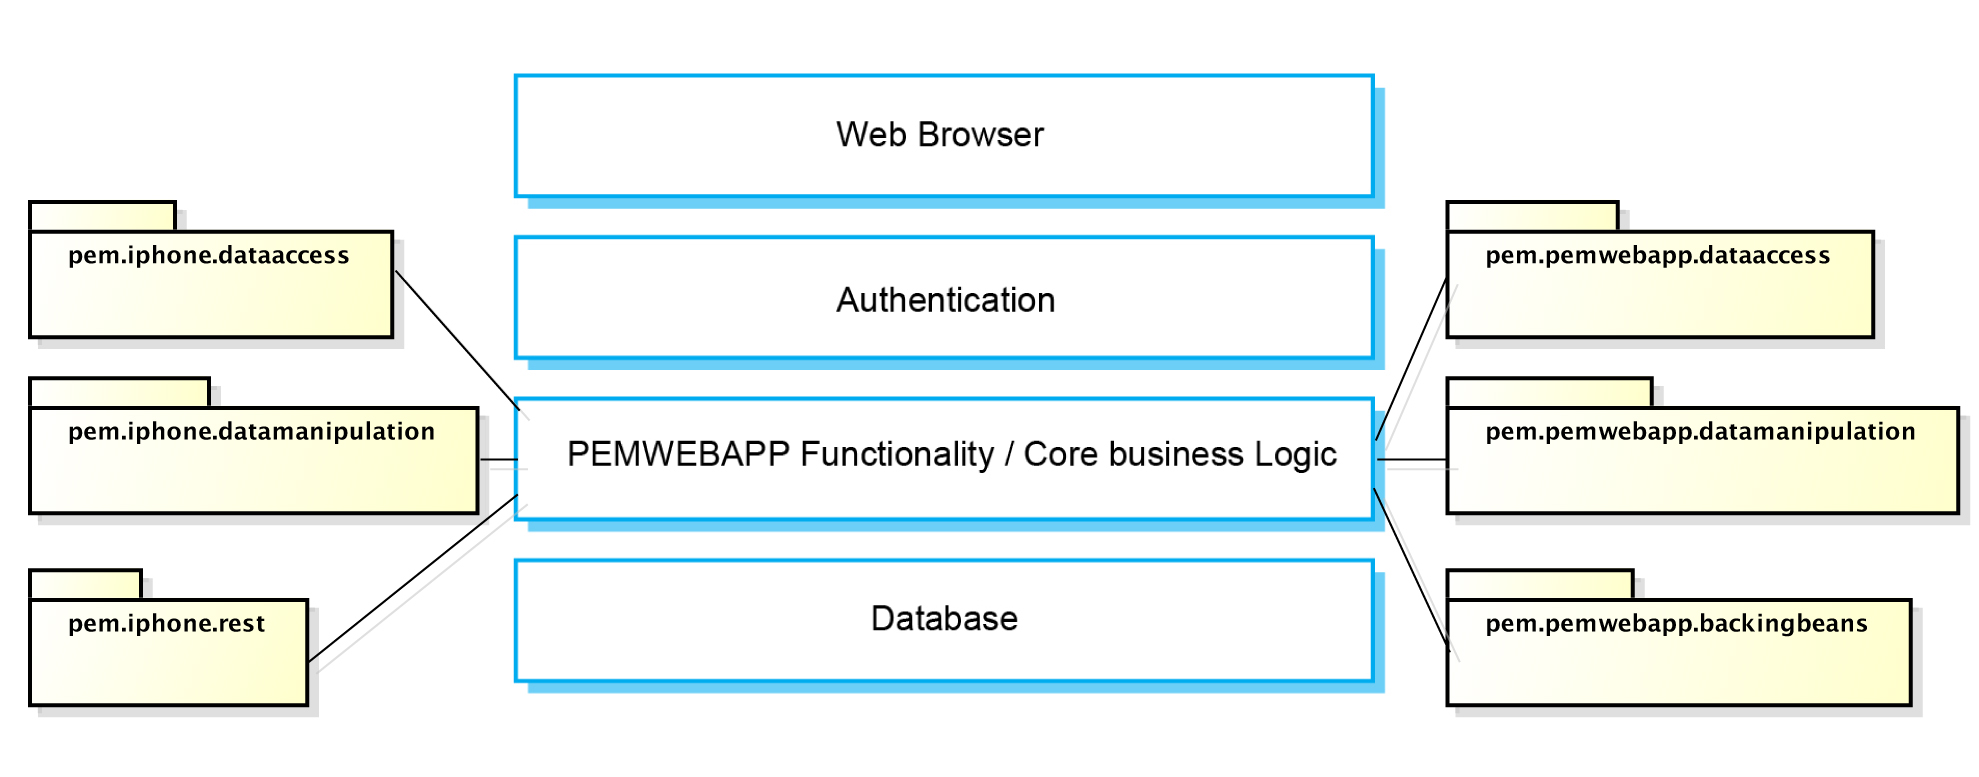
\includegraphics[width=120mm]{/content/PEMWEBAPP-LayeredArchitectureWithPackages.jpg}
	  \caption{PEMWEBAPP layered architecture. Diagram originates from [26] and has been improved to reflect architecture of PEMWEBAPP.}
\end{figure}
 
\clearpage
Both, PEM and PEMWEBAPP will also comply with the Client-server architectural pattern. \\
 
 
\begin{figure}[H]
  \centering
	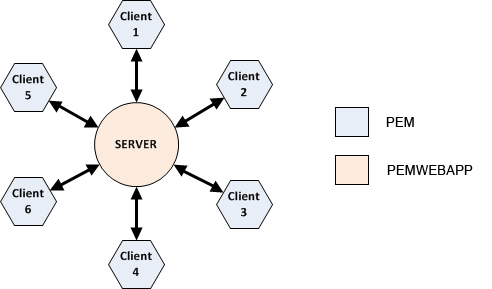
\includegraphics[width=120mm]{/content/client_server.jpg}
	  \caption{Client-server architectural pattern [27]}
\end{figure}
 
 
The design of the PEMWEBAPP was not as complicated as design of the PEM. And therefore the initial architecture outlined, proved to be a simple but solid application as used in enterprise environments.


\begin{figure}[H]
\begin{sideways}
\begin{minipage}{19cm}
	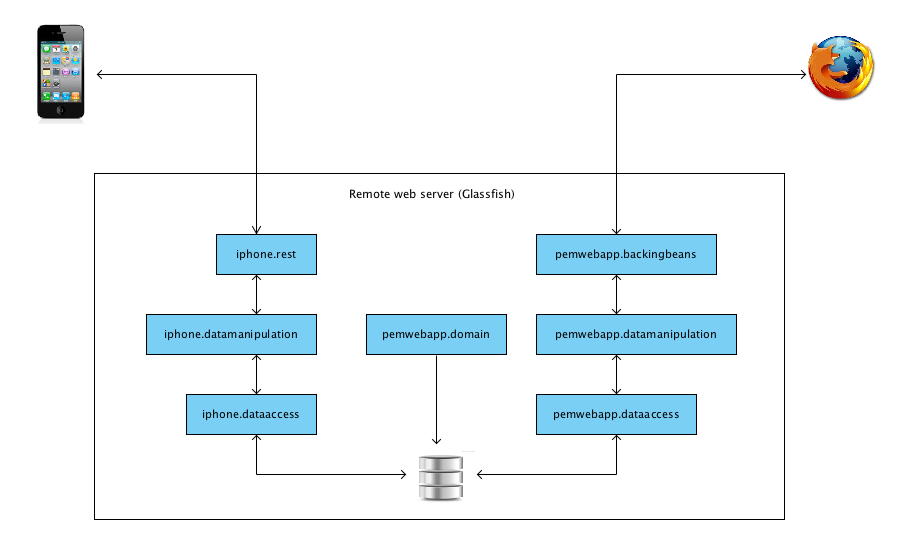
\includegraphics[width=200mm]{/content/pemwebappArchitecture.jpg}
	\caption{Architectural design of PEM and PEMWEBAPP}
\end{minipage}
\end{sideways}
\centering
\end{figure}
 

\clearpage
\subsection{Identifying the principal objects in the system}
For identifying the principal objects in the system a grammatical analysis of a natural language description combined with scenario-based analysis were used. Grammatical analysis in Object-Oriented design is a technique of identifying nouns and verbs. Nouns in the description refer to things (sources of classes and objects) and verbs refer to actions (sources of interactions between objects which can be though of as methods). In scenario-based analysis various scenarios of system are identified and analysed to refine object selection.\\ \\


\subsection{Developing design models}
Following sets of class diagrams show design of most important parts of both systems. Any further development of PEM or PEMWEBAPP can be built on top of these designs.
 

\begin{figure}[H]
\begin{sideways}
\begin{minipage}{19cm}
	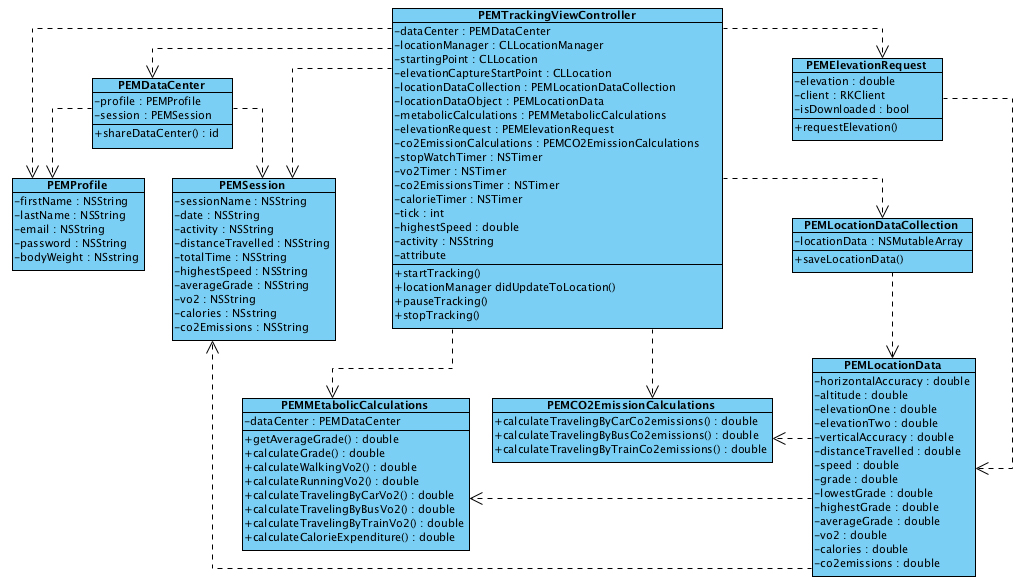
\includegraphics[width=200mm]{/content/PEM-trackingClassDiagram.jpg}
	\caption{PEM's class diagram - design of GPS tracking and data processing}
\end{minipage}
\end{sideways}
\centering
\end{figure}


\begin{figure}[H]
\begin{sideways}
\begin{minipage}{19cm}
	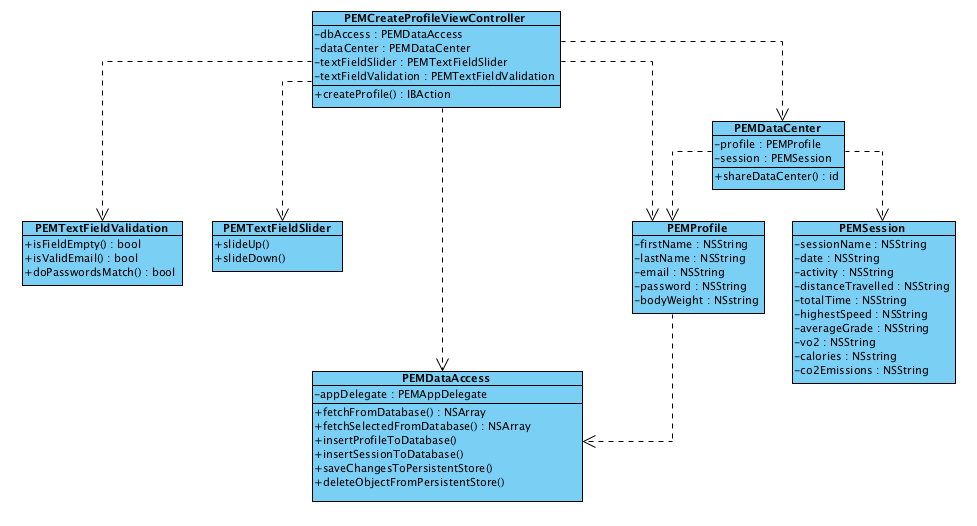
\includegraphics[width=200mm]{/content/PEM-createProfileCD.jpg}
	\caption{PEM's class diagram - design of creating a profile}
\end{minipage}
\end{sideways}
\centering
\end{figure}


\begin{figure}[H]
\begin{sideways}
\begin{minipage}{19cm}
	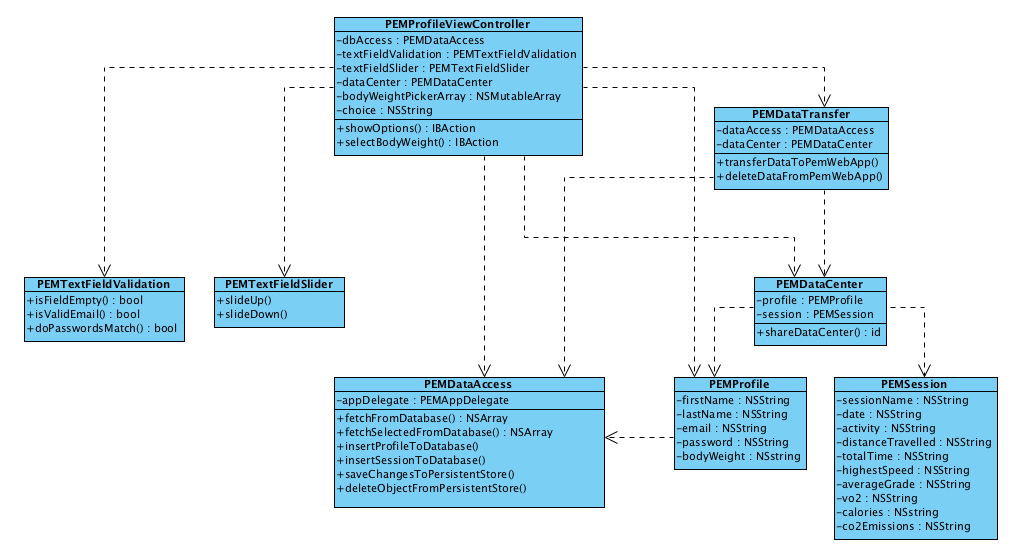
\includegraphics[width=200mm]{/content/PEM-TransferDataCD.jpg}
	\caption{PEM's class diagram - design of data transfer}
\end{minipage}
\end{sideways}
\centering
\end{figure}


\begin{figure}[H]
\begin{sideways}
\begin{minipage}{19cm}
	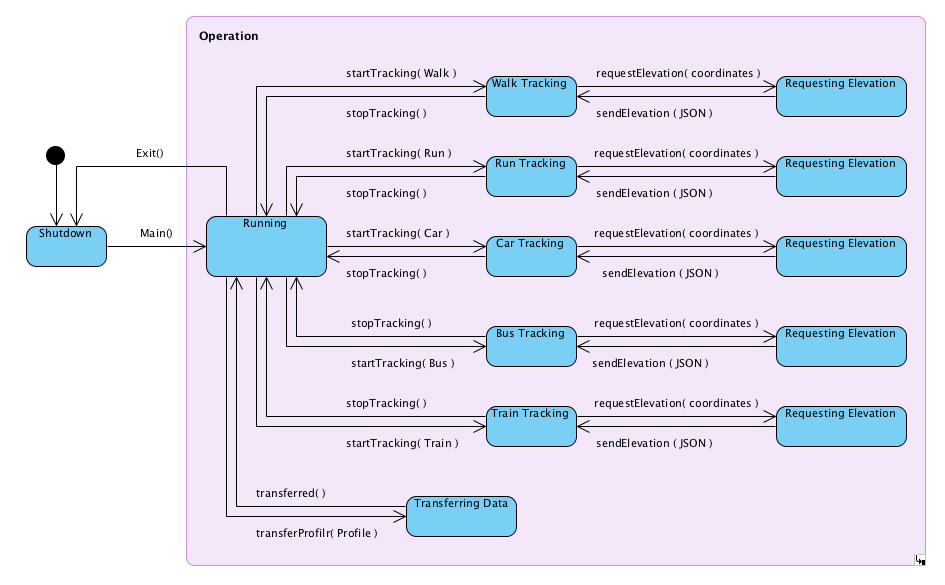
\includegraphics[width=200mm]{/content/PEM-stateDiagram.jpg}
	\caption{PEM's state diagram}
\end{minipage}
\end{sideways}
\centering
\end{figure}


\begin{figure}[H]
\begin{sideways}
\begin{minipage}{19cm}
	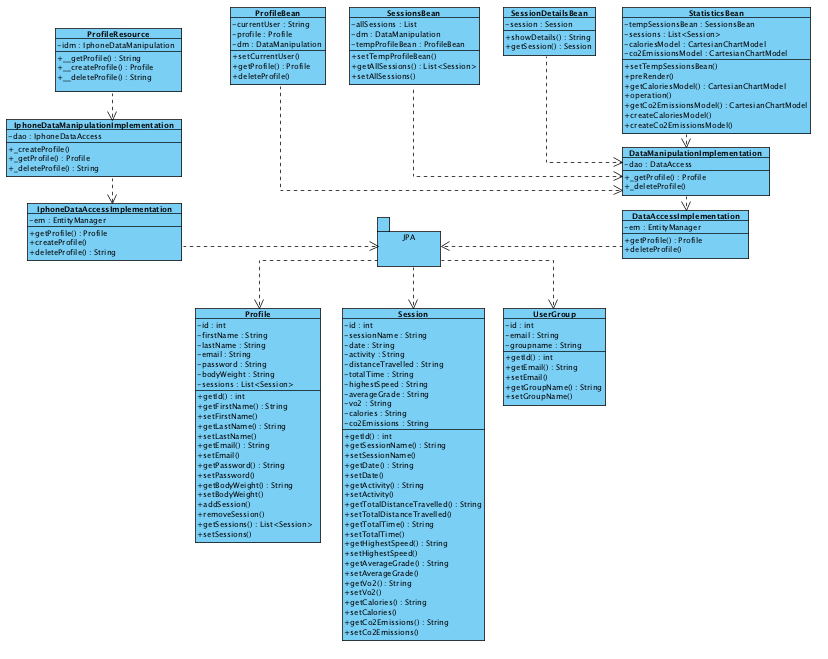
\includegraphics[width=200mm]{/content/PEMWEBAPP-classDiagram.jpg}
\end{minipage}
\end{sideways}
\centering
\caption{PEMWEBAPP's class diagram}
\end{figure}


\subsection{Configuration management}
Software project consists of several documents (files) and together they form a configuration of the project. There is on-going need in a software development life cycle to change documents. If many people work on one particular file they may destroy each others work. This problem can be solved by a technique called version control. In essence it is a version naming scheme and looks, for example, like this:\\


\begin{tabular}{ll}
filename\_v0.0a.txt - (Tom creates a text file)\\
filename\_v0.0b.txt - (Eric adds some content to it)\\
filename\_v0.0c.txt - (Tom replaces some content)\\
filename\_v0.1.txt - (Audited by Tim and checked in)\\
Hannah needs to change the document and proposes the change.\\
The proposal is accepted.\\
filename\_v0.1a.txt - (Hannah check out the file)\\
filename\_v0.1b.txt - (Hannah edits the file)\\
\end{tabular}\\ \\	
	
	
This process can be automated by using a version control system. Versions of both PEM and PEMWEBAPP have been managed by Git. Git is a free and open source, distributed version control system. Distributed means that each user working on a same project has a local repository. Users commit changes to their local repository. Once changes are completed they can push/pull their changes to other remote repositories. This ensures that project changes are being synchronised. As this particular project involved only one developer, myself, there was no need for synchronisation and changes were being pushed to remote GitHub repository only.
With every major change in the project a baseline was created. The baseline is a reviewed and accepted version of a document, from which for all future development is derived.\\ \\
	
	
% Evaluation and Testing
\clearpage
\chapter{Evaluation and Testing}
To ensure that the PEM's metabolic calculations work as intended and produce reasonably accurate results the application had to be evaluated and calculations fine-tuned. The evaluation was done on data that were gathered from PEM's activity monitoring. The data were gathered in the background while the application was running. The following figure~\ref{PEM-evaluation} shows values produced by monitoring a walking activity. Values in the data sheet are produced by GPS tracking and by metabolic calculations.\\


\begin{figure}[H]
\begin{sideways}
\begin{minipage}{19cm}
	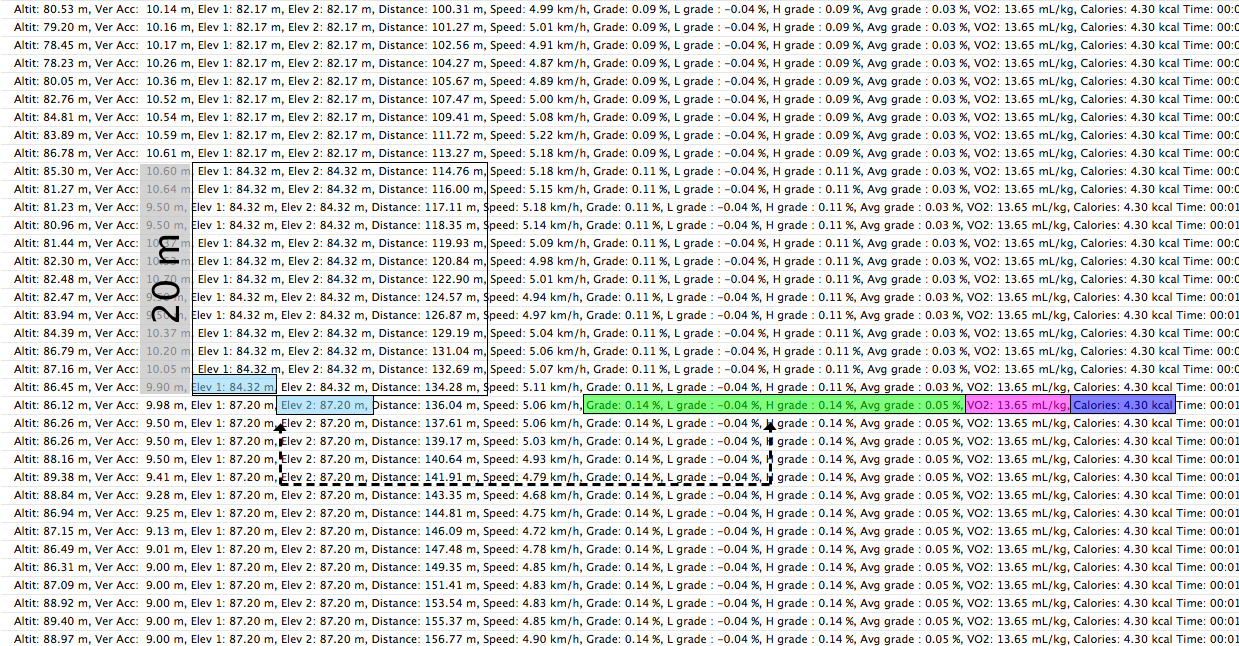
\includegraphics[width=200mm]{/content/PEM-evaluation.jpg}
	\caption{PEM's evaluation data sheet}
	\label{PEM-evaluation}
\end{minipage}
\end{sideways}
\centering
\end{figure}


\clearpage
From the figure~\ref{PEM-evaluation} we can see the different elevation values being collected at two different points. These points have 20 metres between each other. The GPS tracking method knows that it should perform a calculation of grade every 20 meters. Results of this calculation are stored in columns Grade, L Grade (Lowest Grade) and H Grade (Highest Grade). The reason for lowest and highest grade is to calculate an average grade because an individual can walk uphill or downhill many times in a period of time. What we want to achieve is to have one average value of the grade in that period of time.\\ \\
Values in the data sheet show estimates of caloric expenditure of myself with body weight of 63 kg. I have used 13.65 mL/kg of O2 and 4.30 kcal while walking for 01.29 minutes.\\ \\
If compared with a table below, we can see that an individual of a similar weight (145 lbs = 65.7 kg) expends 30 kcal per 5 min, which is 6 kcal per minute.\\


\begin{figure}[H]
  \centering
	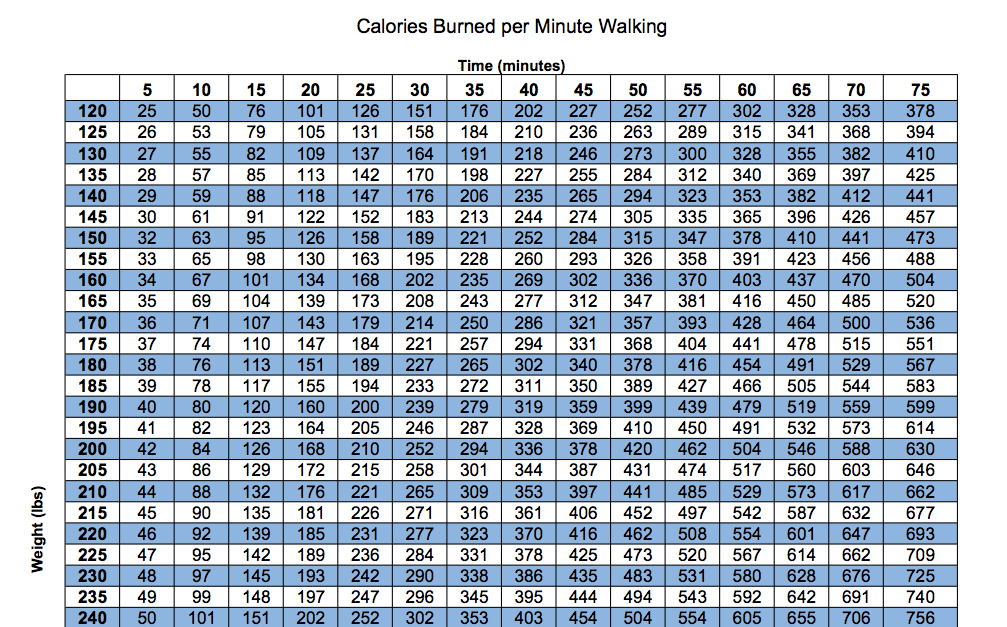
\includegraphics[width=120mm]{/content/CaloriesPerMin.jpg}
	  \caption{Caloric estimates of walking activity produced by Stanford University's Parking and Transportation Services [28]}
\end{figure}


\chapter{Conclusion}
The project has started with high demands and expectations, to develop a product, which would make use of most of the knowledge acquired during the time at university. However the learning curve of iPhone development and JavaEE were unexpectedly steep and there were many unforeseen complications during the development that had to be addressed. Lots of time had to be invested into implementing a basic iPhone application structure and user interface to have a code that compiles and runs correctly.\\ \\
The vast majority of the time was learning the iPhone operating system, Objective-C language and Xcode. There where stages in the development process where concepts such standard data sharing between objects, as it was previously learned with Java, did not work with iPhone development. Linking GUI with logic as it is done with Xcode also wasn't experienced before as well as using delegation and protocols. It turned out that all of them were originating from the strict Apple's adherence to the Model-View-Controller pattern, which had to be learned before any useful iPhone application could be created.
Before any code could be written to implement the PEMWEBAPP, the most time consuming part, was to install and configure the remote server and local machine on which coding was done.
Overall I feel that the coding part of the project was a success. Both applications are working and together with implementing all primary user requirements I have managed to create one of the extensions that required more precise data processing. I have done this with help of the Google Elevation API.\\ \\

I think having chosen to implement the PEM for Android (operating system for mobile devices which runs Java applications) the final result of this project would have better qualities overall. Lots of Java programming experience has been acquired in last three years that would be sufficient for completing more features from the extension section. The time spend on research of iPhone development could be better spent on project planning and time management which were poor. I also wish I have spent time testing the system throughout the development phase rather that prioritising implementation of all user requirements.
Having said that, I am very happy that I have challenged myself to research both of these big topics. Through the hard times in the development I have learned lots of underlying architecture and design patterns that I feel confident enough to start coding iPhone applications and Java web applications commercially.

\section{Future work}
The plan of the future development would be to implement all extensions, but the project has limitless possibilities.  The most important feature to implement would be the secure data transfer. Currently the PEM's data transfer works with no encryption, which violates the Code of Conduct section 1. subsection (a). Further efforts could be focussed for example on utilising the iPhone's accelerometer for gathering motion data and use these data in metabolic calculations. This would be useful in environment without GPS signal of when there is not much location change e.g. running on treadmill or working out on stepper.\\ \\
It would be also interesting to implement the energy expenditure model proposed by Simon Hay, Stamatina Th. Rassia , Alastair Beresford and Nick V. Baker and see how it performs. The PEMWEBAPP could be turned into a social web site where would people share their daily energy expenditure reports thus creating health trends. Similar way it would be possible to see patterns of carbon footprint with granularity of individuals.

\begin{thebibliography}{9}
  % type bibliography here
 
\subsection*{Literature}

\begin{itemize}
	\item [1] David Mark, Jack Nutting, Jeff LaMarche. (2011). Beginning iPhone 4 Development: Exploring the iOS SDK. Apress.\\
	\item [2] Maher Ali. (2010). Advanced iOS 4 Programming: Developing Mobile Applications for Apple iPhone, iPad, and iPod touch
. Wiley\\
	\item [3] Antonio Goncalves. (2010). Beginning Java EE 6 with GlassFish 3 (Expert's Voice in Java Technology). Apress.\\
	\item [4] American College of Sports Medicine. (2006). ACSM's Metabolic Calculations Handbook. Lippincott Williams \& Wilkins. p3.\\
\end{itemize}

\subsection*{Reference}

\begin{itemize}
	\item [1] Wikipedia, Global Positioning System. \url{http://en.wikipedia.org/wiki/Global_Positioning_System}. Last visited 26. April 2012.\\
	\item [2] American College of Sports Medicine. (2006). ACSM's Metabolic Calculations Handbook. Lippincott Williams \& Wilkins. p3.\\
	\item [3] Simon Hay. A global personal energy meter. In Adjunct Proceedings of the 7th International Conference on Pervasive Computing (Pervasive 2009)\\
	\item [4] Carbon Trust. \url{http://www.carbontrust.com/resources/reports/advice/conversion-factors}. Last visited 20. April 2012.\\
	\item [5] Art Knowledge News. \url{http://www.artknowledgenews.com/Leonardo_da_Vinci.html}. Last visited 26 April 2012.\\
	\item [6] Justin Kitzes, Mathis Wackernagel, Jonathan Loh, Audrey Peller, Steven Goldfinger, Deborah Cheng, and Kallin Tea. Shrink and share: humanity's present and future Ecological Footprint. Philos Trans R Soc Lond B Biol Sci. 2008 February 12; 363(1491): 467–475.\\
	\item [7] Global Positioning System. \url{http://en.wikipedia.org/wiki/Global_Positioning_System}. Last visited 16. April 2012.\\
	\item [8] Stamatina Th. Rassia, Simon Hay, Alastair Beresford and Nick Baker. Movement dynamics in office environments. In Proceedings of the 3rd CIB International Conference on Smart and Sustainable Built Environments (SASBE 2009).\\
	\item [9] Simon Hay, Stamatina Th. Rassia and Alastair Beresford. Estimating personal energy expenditure with location data. In Proceedings of the First IEEE PerCom Workshop on Pervasive Healthcare (PerHealth 2010, in conjunction with PerCom 2010).\\
	\item [10] Ian Sommerville. (2010). Software Engineering (9th Edition). Addison Wesley. p73.\\
	\item [11] iOS App Programming Guide. \url{http://developer.apple.com/library/ios/documentation/iphone/conceptual/iphoneosprogrammingguide/iphoneappprogrammingguide.pdf}. Last visited 26. April 2012.\\
	\item [12] Core Location Framework Reference. \url{http://developer.apple.com/library/ios/#documentation/CoreLocation/Reference/CoreLocation_Framework/_index.html#//apple_ref/doc/uid/TP40007123}. Last visited 24. April 2012.\\
	\item [13] iOS App Programming Guide. \url{http://developer.apple.com/library/ios/documentation/iphone/conceptual/iphoneosprogrammingguide/iphoneappprogrammingguide.pdf}. Last visited 22. April 2012.\\
	\item [14] India Curry. \url{http://www.indiacurry.com/weightloss/walkingrunningcalories.htm}. Last visited 05. April 2012.\\
	\item [15] LIVESTRONG. \url{http://www.livestrong.com/article/78365-estimate-calories-burned-heart-rate/}. Last visited 05. April 2012.\\
	\item [16] Stamatina Th. Rassia, Simon Hay, Alastair Beresford and Nick Baker. Movement dynamics in office environments. In Proceedings of the 3rd CIB International Conference on Smart and Sustainable Built Environments (SASBE 2009).\\
	\item [17] School for Champions. \url{http://www.school-for-champions.com/science/work_energy.htm}. Last visited 23. April 2012.
	\item [18] Measurement of Work, Power and Energy Expenditure. \url{http://jan.ucc.nau.edu/pe/exs336web/336workpower.htm}. Last visited 20 April 2012.\\
	\item [19] American College of Sports Medicine. (2006). ACSM's Metabolic Calculations Handbook. Lippincott Williams \& Wilkins. p3.\\
	\item [20] MediKro. \url{http://www.medikro.com/eSupport/index.php?_m=knowledgebase&_a=viewarticle&kbarticleid=35}. Last visited 23. April 2012.\\
	\item [21] Carbon Trust. \url{http://www.carbontrust.com/resources/reports/advice/conversion-factors}. Last visited 20. April 2012.\\
	\item [22] How To Forge.com \url{http://www.howtoforge.com/}. Last visited 10. March 2012.\\
	\item [23] Wikipedia, Dependency injection. \url{http://en.wikipedia.org/wiki/Dependency_injection}. Last visited 24 April 2012.\\
	\item [24] Ian Sommerville. (2010). Software Engineering (9th Edition). Addison Wesley. p178.\\
	\item [25] Ian Sommerville. (2010). Software Engineering (9th Edition). Addison Wesley. p156.\\
	\item [26] Ian Sommerville. (2010). Software Engineering (9th Edition). Addison Wesley. p158.\\
	\item [27] Advanced Object-Oriented Programming and Design. \url{http://www.clear.rice.edu/comp310/f11/lectures/lec26/}. Last visited 22. April 2012. \\
	\item [28] transportation.stanford.edu \url{http://transportation.stanford.edu/pdf/caloriecalc_walk.pdf}. Last visited 24. April 2012
	

\end{itemize}


\end{thebibliography}

\chapter*{Appendices}

\subsubsection{Work log}
04. Sep 2011 - Read the Sussex page on Final year project \\
04. Sep 2011 - Deciding on the project (must have web development and hardware involved)\\
15. Sep 2011 - Started on reading the book on How to do the projects in IT\\
29. Sep 2011 - Decided on the project (PEM, iPone app + Java website)\\
30. Sep 2011 - No Mac (limited resources ), so had to Hackintosh PC to run OSX (Win7 and OSX dualboot netbook)\\
02. Oct 2011 - Installed and configured XCODE IDE\\
03. Oct 2011 - Watched tutorials on iOS development and iPhone SDK technology\\
04. Oct 2011 - Checked and tested most of the available pedometer applications in the AppStore\\
08. Oct 2011 - Registered at Apple Developer Programme, configured iPhone with XCODE\\
09. Oct 2011 - Created my first iPhone app (current position location in Google maps) and transfered it to my iPhone\\
10. Oct 2011 - Read chapter on How to do the projects in IT\\
15. Oct 2011 - Read paper from M. Berger about PEM\\
19. Oct 2011 - Wrote project proposal\\
20. Oct 2011 - Study of iPhone SDK and development guidelines\\
22. Oct 2011 - Study of Lynda.com iPhone Development Essential Training, Gathering literature about GPS, accessing GPS data on iPhone\\
23. Oct 2011 - Created simple GPS application (Capture and display of GPS data on iPhone)\\
24. Oct 2011 - Wrote simple Obective-C console programs\\
25. Oct 2011 - Learning about CoreData\\
30. Oct 2011 - Built app storing data using 4 diffferent approaches\\
01. Nov 2011 - Learning about Core Location\\
02. Nov 2011 - Built app which measures distance. Dealing with accuracy.\\
03. Nov 2011 - First PEM prototype\\
05. Nov 2011 - Improving PEM's accuracy\\
06. Nov 2011 - Implementing PEM's multiview UI\\
09. Nov 2011 - Reading documentation on iPhone View Controllers\\
13. Nov 2011 - Learning to use LeX for writing my report\\
14. Nov 2011 - Writing the Interim Report\\
16. Nov 2011 - Writing the Interim Report\\
17. Nov 2011 - Writing the Interim Report\\
18. Nov 2011 - Researching for planning and organising tools for my project\\
20. Nov 2011 - Upgrading from XCODE 3 to XCODE 4, learning the interface, further study of project planning\\
24. Nov 2011 - Reading iOS App Programming Guide\\
12. Dec 2011 - Building user interface in iOS5 using storyboards (upgrade of the prototype)\\
13. Dec 2011 - Implementing of the CoreData in multi view prototype\\
13. Dec 2011 - Wrote and implemented algorithms for user login and create account features\\

14. Dec 2011 - Implemented user profile management\\
19. Dec 2011 - Refactoring the app\\
21. Dec 2011 - Passing data between two view controllers (Protocol and Delegate)\\
25. Dec 2011 - Sharing data between view controllers (using a singleton pattern)\\
27. Dec 2011 - Building an Action sheet for option selection\\
01. Jan 2012 - Building a sliding picker view for age selection\\
02. Jan 2012 - Research on calorie burn calculation (different ways of estimation)\\
04. Jan 2012 - Changed age to weight in Profile view. Implemented tracking view. Implemented a count up timer\\
02. Feb 2012 - MySQL setup and connecting IDE with database\\
03. Feb 2012 - First Java web application implementd\\
05. Mar 2012 - First PEMWEBAPP prototype\\
20. Mar 2012 - Fine tuning the PEM's GPS\\
07. Apr 2012 - Implemented PEM's data transfer\\
08. Apr 2012 - Finished PEM\\
09. Apr 2012 - Improved PEMWEBAPP' user interface\\
10. Apr 2012 - Utilised the PrimeFaces JSF components\\
11. Apr 2012 - Utilised the PrimeFaces line chart and connected to database\\
12. - 26. Apr 2012 - Writing of the final year report

\end{document}






